\documentclass[11pt]{article}
\usepackage{amsmath,amssymb,amsfonts}
\usepackage{algorithm}
\usepackage{algpseudocode}
\usepackage{gensymb} % For proper degree symbol in math mode
\usepackage{graphicx}
\setlength{\headheight}{13.6pt} % Fix header height warning
\usepackage{textcomp}
\usepackage{xcolor}
\usepackage{caption}
\usepackage{subcaption}
\usepackage{tabularx}
\usepackage{array}
\usepackage{multirow}
\usepackage{geometry}
\usepackage{fancyhdr}
\usepackage{titlesec}
\usepackage{float}
\usepackage{tikz}
\usetikzlibrary{positioning,matrix}
\usepackage{listings}
\usepackage{indentfirst}
\geometry{margin=1in}
\pagestyle{fancy}
\graphicspath{{code/figures/}{../figures/}{figures/}}

% University of South Carolina color palette
\definecolor{USCGarnet}{HTML}{73000A}
\definecolor{USCBlack}{HTML}{000000}
\definecolor{USCRichBlack}{cmyk}{0.4,0.3,0.3,1}
\definecolor{USCWhite}{HTML}{FFFFFF}
\definecolor{USCBlackNinety}{HTML}{363636}
\definecolor{USCBlackSeventy}{HTML}{5C5C5C}
\definecolor{USCBlackFifty}{HTML}{A2A2A2}
\definecolor{USCBlackThirty}{HTML}{C7C7C7}
\definecolor{USCBlackTen}{HTML}{ECECEC}
\definecolor{USCWarmGrey}{HTML}{676156}
\definecolor{USCSandstorm}{HTML}{FFF2E3}
\definecolor{USCRose}{HTML}{CC2E40}
\definecolor{USCAtlantic}{HTML}{466A9F}
\definecolor{USCCongaree}{HTML}{1F414D}
\definecolor{USCHorseshoe}{HTML}{65780B}
\definecolor{USCGrass}{HTML}{CED318}
\definecolor{USCHoneycomb}{HTML}{A49137}
\definecolor{USCDarkGarnet}{HTML}{570008}
\definecolor{USCAzalea}{HTML}{844247}

\lstdefinestyle{uscMatlab}{
  language=Matlab,
  basicstyle=\ttfamily\small\color{USCBlack},
  keywordstyle=\color{USCGarnet}\bfseries,
  commentstyle=\color{USCHorseshoe}\itshape,
  stringstyle=\color{USCAzalea},
  identifierstyle=\color{USCAtlantic},
  numberstyle=\tiny\color{USCHorseshoe},
  backgroundcolor=\color{USCBlackTen},
  rulecolor=\color{USCAtlantic},
  frame=single,
  framerule=0.8pt,
  xleftmargin=1em,
  xrightmargin=1em,
  breaklines=true,
  tabsize=4,
  showstringspaces=false,
  emph={synthetic_ps_min,exp1_poisson_only,exp2_ps_gaussian,rotate_light_shape},emphstyle=\color{USCRose}\bfseries,
  emph={[2]save_heatmap,save_profile,save_hist},emphstyle={[2]\color{USCDarkGarnet}},
  morecomment=[l][\color{USCHoneycomb}]{\%\%}
}
\lstset{style=uscMatlab}

% Single column, no two-column mode
\onecolumn

% Customize title formatting
\titleformat{\section}{\Large\bfseries}{\thesection}{1em}{}
\titleformat{\subsection}{\large\bfseries}{\thesubsection}{1em}{}
\titleformat{\subsubsection}{\normalsize\bfseries}{\thesubsubsection}{1em}{}

% Math operators
\DeclareMathOperator*{\argmin}{arg\,min}

\title{\LARGE\bfseries 3D Surface Reconstruction via the Photometric Stereo Method}

\author{JC Vaught and Ty Dangerfield \\ Department of Mechanical Engineering, University of South Carolina}

\date{\today}

\begin{document}
\maketitle

\begin{abstract}
We present an analytical and numerical validation of the photometric stereo method used in industrial applications for defect detection. This paper details six primary contributions toward a synthetic photometric pipeline: (1) eight unique surface geometries, (2) rigorous mathematical solutions for both numerical and analytical approaches, (3) detailed algorithmic explanations for each primary component of the pipeline, (4) experimental validation across eight shapes and sixteen light-source locations, (5) ablation studies on number of lights, noise robustness, and resolution impacts, and (6) a comparison of two alternative solver methods and their impact on results. Three-dimensional reconstruction depth errors range from 0.022 through 0.147, well within acceptable tolerances and demonstrating robust recovery. Angular errors of the normals reconstruction remain below $3.5\degree$ for smooth surfaces and $2\degree$ for polyhedral shapes.
\end{abstract}

\begin{table}[H]
\centering
\caption{Individual Contributions}
\label{tab:individual_contributions}
\begin{tabular}{ll}
\hline\hline
\textbf{Contribution} & \textbf{Primary Contributor(s)} \\
\hline
MATLAB implementation of complete program & Ty Dangerfield \\
Python implementation of complete program & JC Vaught \\
Photometric principle derivation & Ty Dangerfield \& JC Vaught \\
Gradient integration with Poisson solver & Ty Dangerfield \\
Separation of variables and numerical derivations & JC Vaught \\
Report chapters 1, 3, and 4 (initial) & JC Vaught \\
Report chapters 1, 2, and 5 (initial) & Ty Dangerfield \\
Report restructuring and enhanced documentation & JC Vaught \& Ty Dangerfield \\
Code architecture refinement and expansion & JC Vaught \& Ty Dangerfield \\
\hline\hline
\end{tabular}
\end{table}

\begin{table}[H]
\centering
\caption{Meeting Participation}
\label{tab:meeting_participation}
\begin{tabular}{lcc}
\hline\hline
\textbf{Date} & \textbf{JC Vaught} & \textbf{Ty Dangerfield} \\
\hline
19 Nov 2025 & Present & Present \\
20 Nov 2025 & Present & Present \\
07 Dec 2025 & Present & Present \\
\hline\hline
\end{tabular}
\end{table}

\vspace{1em}
\newpage

\tableofcontents
\newpage

%%%%%%%%%%%%%%%%%%%%%%%%%%%%%%%%%%%%%%%%%%%%%%%%%%%%%%
\section{Introduction}
\label{sec:introduction}

\subsection{What We Want to Model}

Three-dimensional surface reconstruction is a fundamental problem in manufacturing applications and mechanical engineering more broadly. Photometric stereo is one possible solution among many, yielding highly accurate surface reconstruction compared to a dual-camera setup, which is more often used in robotic applications.

Given multiple 2D images of an object illuminated from different directions, we derive the PDE, analytical solution, and numerical solution that create an accurate reconstruction of the 3D depth map or surface geometry.

\subsection{Why This Problem is Important}

Photometric stereo has impact across multiple domains summarized in Table~\ref{tab:ps_applications}, including industrial inspection, where it supports surface defect detection and tolerance verification; medical imaging, where it enables high-fidelity reconstructions of anatomical surfaces for planning; archaeology, where non-destructive digitization preserves fragile artifacts; robotics and autonomous systems, where detailed surface geometry informs grasping and navigation; and reverse engineering, where recovered shapes seed CAD models for subsequent design and analysis.

\begin{table}[H]
\centering
\caption{Representative Application Domains for Photometric Stereo}
\label{tab:ps_applications}
\begin{tabular}{ll}
\hline\hline
\textbf{Domain} & \textbf{Example Use} \\
\hline
Industrial inspection & Surface defect detection, geometric tolerance checks \\
Medical imaging & Preoperative surface reconstruction for planning \\
Archaeology & Non-destructive digitization of artifacts \\
Robotics & Shape-aware grasp planning and manipulation \\
Autonomous vehicles & High-fidelity surface maps for navigation \\
Reverse engineering & Recovering geometry for CAD modeling \\
\hline\hline
\end{tabular}
\end{table}


\noindent Photometric stereo is an ideal solution for many surface extraction tasks owing to the reduction in moving parts. For example, in structure-from-motion methods, the movement of the camera must be precisely monitored and controlled, necessitating careful calibration; even minor calibration errors can severely impact reconstruction quality. Stereo cameras avoid motion but still suffer from calibration issues because the distance, angle, and focal length of each camera---the intrinsic parameters---must be known precisely to estimate depth. Any error there can distort the recovered geometry due to the trigonometric basis of the method. Photometric stereo, on the other hand, is a completely solid-state approach with a single camera, operates at a higher rate than structure-from-motion, and has lower data requirements than stereo systems. Because it leverages illumination direction to infer depth from shading and then reconstruct normals, it is inherently more tolerant to noise and avoids multi-camera calibration drift.

However, photometric stereo does suffer from one critical constraint: the illumination sequence must be precisely controlled. As a result, it cannot be used effectively in uncontrolled environments such as UAVs or general-purpose robotics, which is why stereo cameras remain the de facto standard outside manufacturing despite their calibration sensitivity. Nevertheless, the fundamental challenge in photometric stereo still lies in \textit{integrating} noisy normal estimates into a globally consistent 3D surface, which requires solving a partial differential equation: the \textbf{Poisson equation}.

\subsection{Comparison with Alternative Methods}

Table~\ref{tab:3d_methods_comparison} compares photometric stereo with other common 3D reconstruction techniques across key performance dimensions. The comparison highlights why photometric stereo is particularly well-suited for controlled industrial environments despite requiring specialized lighting infrastructure.

\begin{table}[H]
\centering
\caption{Comparison of 3D Reconstruction Methods}
\label{tab:3d_methods_comparison}
\small
\begin{tabularx}{\textwidth}{>{\raggedright\arraybackslash}p{2.8cm}XXX}
\hline\hline
\textbf{Method} & \textbf{Advantages} & \textbf{Disadvantages} & \textbf{Typical Use Cases} \\
\hline
\textbf{Photometric Stereo} & 
Single camera; high spatial resolution; dense surface normals; solid-state (no moving parts) & 
Requires controlled lighting; assumes Lambertian reflectance; limited to near-field & 
Defect detection, material inspection, quality control \\
\hline
\textbf{Stereo Vision} & 
Passive (no special lighting); works outdoors; real-time capable & 
Requires precise calibration; texture-dependent; ambiguity in textureless regions & 
Robotics, autonomous vehicles, SLAM \\
\hline
\textbf{Structure from Motion} & 
Single camera; scales to large scenes; robust to illumination changes & 
Requires camera motion; computationally intensive; drift accumulation & 
3D scanning, mapping, archaeological digitization \\
\hline
\textbf{Structured Light} & 
High accuracy; active illumination; fast acquisition & 
Sensitive to ambient light; limited range; projector-camera calibration required & 
Industrial metrology, 3D printing, facial scanning \\
\hline
\textbf{Time-of-Flight} & 
Direct depth measurement; real-time; works in low texture & 
Lower resolution; sensitive to multipath reflections; expensive hardware & 
Gesture recognition, indoor navigation, human-computer interaction \\
\hline\hline
\end{tabularx}
\end{table}

\noindent Photometric stereo excels in industrial settings where lighting can be tightly controlled and surface finish is relatively uniform. The method's ability to capture dense normal fields from a single viewpoint makes it ideal for in-line inspection systems where throughput and repeatability are critical. By contrast, methods like stereo vision or time-of-flight are better suited to unstructured environments (e.g., outdoor robotics) where lighting variability and scene dynamics preclude the use of synchronized illumination sequences.

\subsection{The Core PDE Problem}
The fundamental problem reduces to solving the 2D Poisson equation in a rectangular domain:
\begin{equation}\label{eq:poisson_main}
\nabla^2 z(x,y) = f(x,y), \quad (x,y) \in \Omega = [0, L_x] \times [0, L_y]
\end{equation}
where 
\begin{align*}
z(x,y) &= \text{unknown surface height over the image domain} \\
f(x,y) &= \frac{\partial p}{\partial x} + \frac{\partial q}{\partial y} \quad \text{(divergence of Poisson-derived gradient estimates)} \\
\Omega &= [0,L_x]\times[0,L_y] \quad \text{(rectangular image domain)}
\end{align*}

This project demonstrates both analytical (separation of variables) and numerical (FFT-based and finite-difference) methods to solve this fundamental PDE and validate the solutions on synthetic 3D surfaces.



%%%%%%%%%%%%%%%%%%%%%%%%%%%%%%%%%%%%%%%%%%%%%%%%%%%%%%
\section{Mathematical Foundation}
\label{sec:mathematical_foundation}

This chapter establishes the theoretical foundations for photometric stereo reconstruction. We begin with the photometric stereo principle, deriving the relationship between observed image intensities and surface normals under Lambertian reflectance. We then formulate the gradient integration problem as a Poisson equation, providing both variational and Euler-Lagrange derivations. Next, we develop the theory of boundary conditions---Dirichlet, Neumann, and periodic---and their impact on solution uniqueness. Finally, we present an analytical solution via separation of variables, including eigenfunction expansions and worked examples that validate our numerical methods.

\subsection{Photometric Stereo Principle}

Photometric stereo recovers surface normals from multiple images of a static scene illuminated by different light sources. The key insight is that shading variations across images encode the local surface orientation. Table~\ref{tab:ps_assumptions} summarizes the key modeling assumptions underlying this approach.

\begin{table}[H]
\centering
\caption{Photometric Stereo Modeling Assumptions}
\label{tab:ps_assumptions}
\begin{tabularx}{\textwidth}{>{\bfseries}p{5cm}X}
\hline\hline
\textbf{Assumption} & \textbf{Description} \\
\hline
Lambertian reflectance & Surface reflects light diffusely in all directions; no specular highlights or glossy reflections \\
\hline
Orthographic projection & Camera uses parallel projection (unit focal length); no perspective distortion \\
\hline
Known light directions & Light source directions $\mathbf{L}_i$ are calibrated and known a priori \\
\hline
Static scene & Surface geometry and camera remain fixed across all images \\
\hline
Uniform albedo & In our derivations, albedo $\rho(x,y)$ is assumed constant, though the general formulation allows spatially varying albedo \\
\hline
No inter-reflections & Light reaches the surface directly without bouncing off other surfaces \\
\hline
Attached shadows only & Self-shadowing is handled via the $\max$ operator; cast shadows from other objects are not modeled \\
\hline\hline
\end{tabularx}
\end{table}

\subsubsection{Image Formation Model}

By assuming an ideal camera with a unit focal length, we map a 3D point $\mathbf{X}$ to image coordinates $\mathbf{x}=(x,y)$ for any arbitrary surface with depth $z(x,y)$. 
The measured image intensity $I_i$ at pixel $(x,y)$ under light source $i$ is the product of three components: the camera calibration factor $\kappa_i$ (encapsulating exposure, gain, and light source intensity), the material albedo $\rho(x,y) \in [0,1]$ (the fraction of light reflected by the surface), and the geometric factor $\max\!\bigl(0, \mathbf{n}(x,y) \cdot \mathbf{L}_i\bigr)$ (the cosine of the angle between the surface normal $\mathbf{n}$ and light direction $\mathbf{L}_i$). These combine to yield the image formation equation:
\begin{equation}
I_i(x,y) = \kappa_i\, \rho(x,y) \max\!\bigl(0, \mathbf{n}(x,y) \cdot \mathbf{L}_i\bigr)
\label{eq:imageformation}
\end{equation}
The $\max$ operator enforces attached shadows: when a light illuminates the surface from behind ($\mathbf{n} \cdot \mathbf{L}_i < 0$), the contribution is zero.

\subsubsection{Lambertian Reflectance}

The Lambertian assumption states that a surface appears equally bright from all viewing directions---light is reflected diffusely in all directions. Mathematically, the reflected radiance is proportional to $\cos\theta = \mathbf{n} \cdot \mathbf{L}$, where $\theta$ is the angle between the surface normal and the incident light direction.

To connect surface geometry to shading, we must express the surface normal in terms of the depth map $z(x,y)$. We begin by computing the tangent vectors to the surface. These tangent vectors represent the local orientation of the surface along the $x$ and $y$ coordinate directions:
\begin{align}
\frac{\partial \mathbf{X}}{\partial x} &= (1, 0, p), \quad \text{where } p = \frac{\partial z}{\partial x} \\
\frac{\partial \mathbf{X}}{\partial y} &= (0, 1, q), \quad \text{where } q = \frac{\partial z}{\partial y}
\end{align}
Here, $p$ and $q$ represent the local slopes of the surface in the $x$ and $y$ directions, respectively. Note that the first two components of each tangent vector are $(1,0)$ and $(0,1)$ because we move one unit along the respective image coordinate while the surface height changes by $p$ or $q$.

The surface normal is perpendicular to both tangent vectors and can be computed via their cross product:
\begin{equation}
\tilde{\mathbf{n}} = \frac{\partial \mathbf{X}}{\partial x} \times \frac{\partial \mathbf{X}}{\partial y} = (-p, -q, 1)
\end{equation}
This unnormalized normal $\tilde{\mathbf{n}}$ points away from the surface but does not necessarily have unit length. The negative signs on $p$ and $q$ arise naturally from the cross product and ensure the normal points outward (away from the surface) rather than inward.

To obtain a unit normal vector (required for computing the geometric factor $\mathbf{n} \cdot \mathbf{L}$), we divide by the magnitude:
\begin{equation}
\mathbf{n} = \frac{\tilde{\mathbf{n}}}{\|\tilde{\mathbf{n}}\|} = \frac{(-p,-q,1)}{\sqrt{p^2+q^2+1}}
\label{eq:normalfrompq}
\end{equation}

Equation~\eqref{eq:normalfrompq} explicitly links the integrable gradient field $(p,q)$ to the observed shading---this is the key relationship that enables gradient recovery from images.

\subsubsection{The Linear System Formulation}

Having established the relationship between surface normals and image intensities, we now formulate the inverse problem: given multiple images under different illumination, recover the surface normal at each pixel.

We introduce the scaled normal vector $\mathbf{g}(x,y) = \rho(x,y)\mathbf{n}(x,y)$, which combines the geometric information (normal direction) with the material property (albedo). This factorization is convenient because $\mathbf{g}$ appears linearly in the image formation equation.

Substituting the Lambertian reflectance model~\eqref{eq:normalfrompq} into the image formation equation~\eqref{eq:imageformation}, we obtain for a single light source $i$:
\begin{equation}
I_i(x,y) = \kappa_i \mathbf{L}_i^T \mathbf{g}(x,y)
\end{equation}
where we have absorbed the $\max$ operator into the formulation (assuming no self-shadowing for now; we address this later). This is a scalar equation linear in $\mathbf{g}$.

For $m$ different light sources, we obtain $m$ such equations at each pixel. Stacking these into a single matrix equation yields:
\begin{equation}
\underbrace{\begin{bmatrix}
I_1(x,y) \\
I_2(x,y) \\
\vdots \\
I_m(x,y)
\end{bmatrix}}_{\mathbf{I}(x,y) \in \mathbb{R}^m}
=
\underbrace{\begin{bmatrix}
\kappa_1 \mathbf{L}_1^T \\
\kappa_2 \mathbf{L}_2^T \\
\vdots \\
\kappa_m \mathbf{L}_m^T
\end{bmatrix}}_{S \in \mathbb{R}^{m\times 3}}
\underbrace{\mathbf{g}(x,y)}_{\in \mathbb{R}^3}
\end{equation}

Compactly, we write:
\begin{equation}
S \mathbf{g}(x,y) = \mathbf{I}(x,y)
\label{eq:pslinear}
\end{equation}

The matrix $S$ is called the \textit{illumination matrix} and depends only on the known light directions and calibration factors. The vector $\mathbf{I}(x,y)$ contains the observed intensities, and our goal is to solve for $\mathbf{g}(x,y)$ at every pixel. For a unique solution to exist, $S$ must have full column rank: $\text{rank}(S) = 3$. This requires at least three images ($m \geq 3$) with non-coplanar light directions. In practice, we use $m > 3$ to obtain an overdetermined system, which provides robustness against noise.

\subsubsection{Least-Squares Solution via Pseudoinverse}

When $m > 3$, the system~\eqref{eq:pslinear} is overdetermined and generally has no exact solution due to measurement noise. We instead seek the least-squares solution that minimizes the residual:
\begin{equation}
\hat{\mathbf{g}}(x,y) = \argmin_{\mathbf{g}} \|S\mathbf{g} - \mathbf{I}(x,y)\|_2^2
\end{equation}
Expanding the objective function:
\begin{equation}
\|S\mathbf{g} - \mathbf{I}\|_2^2 = (S\mathbf{g} - \mathbf{I})^T(S\mathbf{g} - \mathbf{I}) = \mathbf{g}^T S^T S \mathbf{g} - 2\mathbf{I}^T S \mathbf{g} + \mathbf{I}^T\mathbf{I}
\end{equation}
Taking the gradient with respect to $\mathbf{g}$ and setting it to zero yields the \textit{normal equations}:
\begin{equation}
\nabla_{\mathbf{g}} \|S\mathbf{g} - \mathbf{I}\|_2^2 = 2S^TS\mathbf{g} - 2S^T\mathbf{I} = 0 \quad \Rightarrow \quad S^TS\mathbf{g} = S^T\mathbf{I}
\end{equation}
Assuming $S$ has full column rank, $S^TS$ is invertible, and we obtain:
\begin{equation}
\mathbf{g}(x,y) = \underbrace{(S^TS)^{-1}S^T}_{S^+ \text{ (pseudoinverse)}} \mathbf{I}(x,y)
\label{eq:leastSquares}
\end{equation}
The matrix $S^+ = (S^TS)^{-1}S^T$ is the Moore--Penrose pseudoinverse of $S$. This solution minimizes the $L^2$ norm of the residual and is unique when $\text{rank}(S) = 3$. Once $\mathbf{g}(x,y)$ is computed, we recover the unit normal and albedo by exploiting the factorization $\mathbf{g} = \rho\mathbf{n}$:
\begin{align}
\hat{\rho}(x,y) &= \|\mathbf{g}(x,y)\|_2 \\
\hat{\mathbf{n}}(x,y) &= \frac{\mathbf{g}(x,y)}{\|\mathbf{g}(x,y)\|_2}
\end{align}
The \textit{direction} of $\mathbf{g}$ encodes the surface normal while its \textit{magnitude} equals the albedo.

\subsubsection{Conditioning and Noise Sensitivity}

The accuracy of the recovered normals depends critically on the \textit{condition number} of $S$:
\begin{equation}
\kappa(S) = \frac{\sigma_{\max}(S)}{\sigma_{\min}(S)}
\end{equation}
where $\sigma_{\max}$ and $\sigma_{\min}$ are the largest and smallest singular values of $S$, respectively. To understand the impact of conditioning, consider the singular value decomposition (SVD) of $S$:
\begin{equation}
S = U\Sigma V^T
\end{equation}
where $U \in \mathbb{R}^{m \times 3}$ and $V \in \mathbb{R}^{3 \times 3}$ are orthogonal matrices, and $\Sigma = \text{diag}(\sigma_1, \sigma_2, \sigma_3)$ contains the singular values in descending order. The pseudoinverse can be expressed as:
\begin{equation}
S^+ = V\Sigma^{-1}U^T
\end{equation}
If the measured intensities contain noise $\Delta \mathbf{I}$ such that $\|\Delta \mathbf{I}\| / \|\mathbf{I}\| = \epsilon$, the relative error in the recovered $\mathbf{g}$ is bounded by:
\begin{equation}
\frac{\|\Delta \mathbf{g}\|}{\|\mathbf{g}\|} \leq \kappa(S) \cdot \epsilon
\end{equation}
This shows that the condition number $\kappa(S)$ controls the worst-case amplification of measurement noise. A large condition number indicates that small errors in $\mathbf{I}$ can lead to large errors in $\mathbf{g}$. To minimize noise sensitivity, we seek to minimize $\kappa(S)$, or equivalently, maximize $\sigma_{\min}(S)$. This is achieved when the light directions $\{\mathbf{L}_i\}$ are uniformly distributed over the unit sphere, ensuring that the columns of $S$ span $\mathbb{R}^3$ evenly. In practice, lights are often arranged in a hemispherical configuration with uniform azimuthal and elevation spacing. Using $m > 3$ images provides two additional benefits: the least-squares solution averages out random noise, and the system becomes more robust to individual measurements corrupted by saturation or outliers.


\subsubsection{Shadow Handling and Robust Estimation}

The linear system~\eqref{eq:pslinear} assumes that all lights illuminate the surface from the front ($\mathbf{n} \cdot \mathbf{L}_i > 0$). When a light source illuminates from behind, \textit{self-shadowing} occurs, and the image formation equation becomes:
\begin{equation}
I_i(x,y) = 0 \quad \text{if } \mathbf{n}(x,y) \cdot \mathbf{L}_i < 0
\end{equation}
These shadowed measurements violate the linear model and must be excluded. The standard approach is to first identify light sources $i$ for which $I_i(x,y) \approx 0$ (or below a threshold), then remove the corresponding rows from $S$ and entries from $\mathbf{I}(x,y)$, and finally solve the reduced least-squares problem on the remaining valid measurements. This row deletion strategy preserves the least-squares structure and ensures that only valid measurements contribute to the normal estimate. However, it requires at least three non-shadowed lights at every pixel to maintain $\text{rank}(S) = 3$.

For pixels near shadow boundaries where intensities are low but non-zero, a weighted least-squares approach provides a smoother alternative:
\begin{equation}
\hat{\mathbf{g}} = \argmin_{\mathbf{g}} \sum_{i=1}^m w_i (I_i - \kappa_i \mathbf{L}_i^T \mathbf{g})^2
\end{equation}
where weights $w_i$ are set based on confidence (e.g., $w_i = \max(0, \mathbf{n} \cdot \mathbf{L}_i)$ or based on intensity magnitude). This provides a smooth transition between fully illuminated and shadowed regions.


%%%%%%%%%%%%%%%%%%%%%%%%%%%%%%%%%%%%%%%%%%%%%%%%%%%%%%
\subsection{Gradient Integration via Poisson Equation}

We now have the normals $\mathbf{g}(x,y)$ from photometric stereo, but our ultimate goal is a height map $z(x,y)$. 
The normals allow us to compute gradient estimates $(p,q) = (\partial z/\partial x, \partial z/\partial y)$, but real measurements are noisy and generally not integrable---the curl $\partial_y p - \partial_x q \neq 0$. 
This section develops the variational framework that projects noisy gradients onto the closest integrable field.

\subsubsection{Variational Formulation}

Given noisy gradient estimates $(\hat{p}, \hat{q})$ from photometric stereo, we seek a height field $z(x,y)$ whose gradients best match the measurements in a least-squares sense. This leads to the variational problem:
\begin{equation}
\min_{z} \; \mathcal{E}[z] = \iint_\Omega \left[(\partial_x z - \hat{p})^2 + (\partial_y z - \hat{q})^2\right] dx \, dy
\label{eq:poisson_variational}
\end{equation}
The functional $\mathcal{E}[z]$ measures the total squared error between the true gradients $(\partial_x z, \partial_y z)$ of the unknown surface and the measured estimates $(\hat{p}, \hat{q})$. By minimizing over all possible height functions $z$, we find the surface whose gradients are closest to the measurements in the $L^2$ norm.

The integrand $\mathcal{L} = (\partial_x z - \hat{p})^2 + (\partial_y z - \hat{q})^2$ depends on $z$ only through its first derivatives $z_x = \partial_x z$ and $z_y = \partial_y z$. This structure is characteristic of problems in the calculus of variations, and the minimizer satisfies the Euler--Lagrange equation.

\subsubsection{Euler--Lagrange Derivation}

For a functional of the form $\mathcal{E}[z] = \iint \mathcal{L}(z, z_x, z_y) \, dx\,dy$, the necessary condition for a minimum is the Euler--Lagrange equation:
\begin{equation}
\frac{\partial \mathcal{L}}{\partial z} - \frac{\partial}{\partial x}\left(\frac{\partial \mathcal{L}}{\partial z_x}\right) - \frac{\partial}{\partial y}\left(\frac{\partial \mathcal{L}}{\partial z_y}\right) = 0
\end{equation}
Since our Lagrangian $\mathcal{L} = (z_x - \hat{p})^2 + (z_y - \hat{q})^2$ does not depend on $z$ directly, we have $\partial \mathcal{L}/\partial z = 0$. Computing the remaining partial derivatives:
\begin{equation}
\frac{\partial \mathcal{L}}{\partial z_x} = 2(z_x - \hat{p}), \qquad \frac{\partial \mathcal{L}}{\partial z_y} = 2(z_y - \hat{q})
\end{equation}
Substituting into the Euler--Lagrange equation:
\begin{equation}
\frac{\partial}{\partial x}\bigl[2(z_x - \hat{p})\bigr] + \frac{\partial}{\partial y}\bigl[2(z_y - \hat{q})\bigr] = 0
\end{equation}
Expanding and rearranging:
\begin{equation}
\partial_x^2 z + \partial_y^2 z = \partial_x \hat{p} + \partial_y \hat{q}
\end{equation}
This is the Poisson equation:
\begin{equation}
\nabla^2 z = f(x,y), \qquad \text{where } f = \nabla \cdot (\hat{p}, \hat{q}) = \frac{\partial \hat{p}}{\partial x} + \frac{\partial \hat{q}}{\partial y}
\label{eq:poisson}
\end{equation}
Here $\nabla^2 = \partial_x^2 + \partial_y^2$ is the Laplacian operator and $f(x,y)$ is the divergence of the measured gradient field. The Poisson equation~\eqref{eq:poisson} arises because an integrable vector field must be curl-free ($\partial_y \hat{p} - \partial_x \hat{q} = 0$). When the measured gradients violate this condition due to noise, solving the Poisson problem projects $(\hat{p}, \hat{q})$ onto the closest integrable field in the $L^2$ sense.

%%%%%%%%%%%%%%%%%%%%%%%%%%%%%%%%%%%%%%%%%%%%%%%%%%%%%%
\subsection{Boundary Condition Theory}

The Poisson equation $\nabla^2 z = f$ admits a unique solution only when supplemented with boundary conditions on $\partial\Omega$. We consider three types that arise in surface reconstruction: Dirichlet, Neumann, and periodic conditions. 
The choice of boundary conditions depends on the physical assumptions about the surface at the image boundary and impacts both solution uniqueness and numerical implementation.

\subsubsection{Dirichlet Boundary Conditions}

Dirichlet conditions prescribe the solution value on the boundary:
\begin{equation}
z(x,y) = g(x,y), \quad (x,y) \in \partial\Omega
\end{equation}
where $g$ is a given function. In the homogeneous case $g \equiv 0$, the surface is pinned to zero height along the entire boundary. This is appropriate when the reconstructed object is known to be flat at the image edges or when the object of interest is contained entirely within the interior of the domain.

For photometric stereo, homogeneous Dirichlet conditions assume that the surface height is zero (or a known constant) at the image boundary. This is suitable for objects that sit on a flat background plane or when the region of interest is masked to exclude edge artifacts. Dirichlet problems always have a unique solution given smooth data.

\subsubsection{Neumann Boundary Conditions}

Neumann conditions prescribe the normal derivative at the boundary:
\begin{equation}
\frac{\partial z}{\partial n}\bigg|_{\partial\Omega} = h(x,y), \quad (x,y) \in \partial\Omega
\end{equation}
where $\mathbf{n}$ is the outward unit normal to $\partial\Omega$ and $h$ specifies the boundary flux. The homogeneous case $h \equiv 0$ imposes zero normal derivative, meaning the surface approaches the boundary with zero slope in the perpendicular direction.

Zero-flux Neumann conditions arise when we have no information about the surface beyond the image boundary. The natural continuation of the gradient field is to assume it stays flat, preventing artificial discontinuities. However, Neumann conditions leave the solution determined only up to an additive constant---we can recover the surface shape but not its absolute height. This lack of absolute height information is resolved by simply setting the average of the entire reconstructed depth profile to zero.

\subsubsection{Periodic Boundary Conditions}

Periodic conditions impose that the solution and its derivatives wrap around at opposite boundaries:
\begin{equation}
z(0, y) = z(L_x, y), \quad z(x, 0) = z(x, L_y), \quad \text{and similarly for derivatives}
\end{equation}
This condition arises naturally when using Fourier-based (FFT) solvers, which assume the domain tiles infinitely in all directions. Under periodicity, the Discrete Fourier Transform diagonalizes the Laplacian operator, enabling $\mathcal{O}(N \log N)$ solution complexity.

Periodic conditions are rarely physical for real surfaces but are computationally convenient. They work well when the surface gradients decay to zero near the boundary (e.g., smooth objects centered in the image) but can introduce artifacts when the surface value or gradient differs significantly between opposite edges. In practice, we often accept these artifacts in exchange for FFT solver speed, especially when the object of interest is well-separated from the image boundary.

\subsubsection{Compatibility and Uniqueness}

The three boundary condition types have different uniqueness and compatibility properties, which determine when a solution exists and whether it is unique up to an additive constant.

\textit{Dirichlet conditions} guarantee a unique solution for any smooth right-hand side $f$ and boundary data $g$. No additional constraints are required---the boundary values fully determine the solution.

\textit{Neumann conditions} require a compatibility constraint. Applying the divergence theorem to the Poisson equation:
\begin{equation}
\iint_\Omega \nabla^2 z \, dA = \oint_{\partial\Omega} \frac{\partial z}{\partial n} \, ds
\end{equation}
Substituting $\nabla^2 z = f$ and the Neumann condition $\partial z/\partial n = h$:
\begin{equation}
\iint_\Omega f \, dA = \oint_{\partial\Omega} h \, ds
\end{equation}
For homogeneous Neumann conditions ($h = 0$), solvability requires:
\begin{equation}
\iint_\Omega f \, dA = 0
\end{equation}
In other words, the source term must integrate to zero over the domain. Even when this condition is satisfied, the solution is unique only up to an additive constant---any $z + c$ is also a solution. We select the unique solution with zero mean.

\textit{Periodic conditions} have the same compatibility requirement as homogeneous Neumann. Since the domain wraps around with no boundary flux, the integral constraint $\iint f \, dA = 0$ must hold. In the FFT formulation, this corresponds to the DC component $\hat{F}[0,0] = 0$---the zero-frequency Fourier coefficient must vanish. The FFT solver enforces this by setting $\hat{F}[0,0] = 0$ before division by the eigenvalues. Like Neumann, periodic conditions also leave an additive constant ambiguity, resolved by zero-mean normalization.


%%%%%%%%%%%%%%%%%%%%%%%%%%%%%%%%%%%%%%%%%%%%%%%%%%%%%%
\subsection{Analytical Solution via Separation of Variables}

Before developing numerical integration schemes to solve the Poisson equation for our photometric stereo application, we first derive an analytical solution as a baseline for comparison---and, candidly, as an exercise to demonstrate mathematical rigor in the realm of partial differential equations. 

The method of separation of variables yields closed-form expressions for problems with homogeneous boundary conditions on rectangular domains. By expanding the solution as a sum of orthogonal eigenfunctions, we obtain exact modal coefficients that serve as ground truth for validating numerical implementations. This section provides the theoretical foundation but will not be directly referenced in subsequent chapters; nevertheless, the analytical benchmark remains essential for verifying solver correctness during development.

\subsubsection{Eigenfunction Expansion}

Consider the 2D Poisson equation on a rectangular domain $\Omega = [0, L_x] \times [0, L_y]$ with homogeneous Dirichlet boundary conditions:
\begin{equation}
\nabla^2 z = f(x,y), \quad (x,y) \in \Omega, \quad z|_{\partial \Omega} = 0
\end{equation}
Using separation of variables, we assume $z(x,y) = X(x)Y(y)$. The homogeneous boundary conditions require $X(0) = X(L_x) = 0$ and $Y(0) = Y(L_y) = 0$, which are satisfied by sine functions. The solution can be written as an eigenfunction expansion:
\begin{equation}
z(x,y) = \sum_{m=1}^{\infty}\sum_{n=1}^{\infty} A_{mn} \sin\left(\frac{m\pi x}{L_x}\right) \sin\left(\frac{n\pi y}{L_y}\right)
\end{equation}

Figure~\ref{fig:modes} illustrates how higher modes introduce additional oscillations. In one dimension, $\sin(m\pi x/L)$ has $m$ half-cycles across the domain, so higher $m$ values correspond to finer spatial detail.

\begin{figure}[h]
\centering
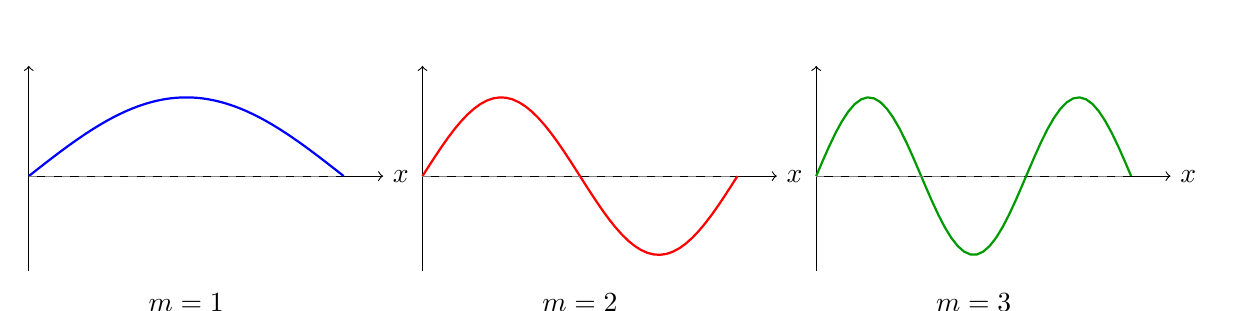
\begin{tikzpicture}[scale=1]
% m=1
\begin{scope}[xshift=0cm]
\draw[->] (0,0) -- (4.5,0) node[right] {$x$};
\draw[->] (0,-1.2) -- (0,1.4);
\draw[thick,blue] plot[domain=0:4,samples=50] (\x,{sin(45*\x)});
\draw[dashed,gray] (0,0) -- (4,0);
\node at (2,-1.6) {$m=1$};
\end{scope}
% m=2
\begin{scope}[xshift=5cm]
\draw[->] (0,0) -- (4.5,0) node[right] {$x$};
\draw[->] (0,-1.2) -- (0,1.4);
\draw[thick,red] plot[domain=0:4,samples=50] (\x,{sin(90*\x)});
\draw[dashed,gray] (0,0) -- (4,0);
\node at (2,-1.6) {$m=2$};
\end{scope}
% m=3
\begin{scope}[xshift=10cm]
\draw[->] (0,0) -- (4.5,0) node[right] {$x$};
\draw[->] (0,-1.2) -- (0,1.4);
\draw[thick,green!60!black] plot[domain=0:4,samples=50] (\x,{sin(135*\x)});
\draw[dashed,gray] (0,0) -- (4,0);
\node at (2,-1.6) {$m=3$};
\end{scope}
\end{tikzpicture}
\caption{Eigenfunctions $\sin(m\pi x/L)$ for $m=1,2,3$. The 2D eigenfunctions are products: $\sin(m\pi x/L_x)\sin(n\pi y/L_y)$. Higher modes oscillate more rapidly and contribute less to the solution because their eigenvalues $\lambda_{mn} \propto m^2 + n^2$ appear in the denominator.}
\label{fig:modes}
\end{figure}

The eigenfunctions form an orthonormal basis for the solution space. Each eigenfunction satisfies the Laplacian eigenvalue problem with eigenvalue $-\lambda_{mn}$ where:
\begin{equation}
\lambda_{mn} = \frac{m^2\pi^2}{L_x^2} + \frac{n^2\pi^2}{L_y^2}
\end{equation}
Substituting the expansion into the Poisson equation and projecting onto each eigenfunction yields the modal amplitudes:
\begin{equation}
A_{mn} = -\frac{F_{mn}}{\lambda_{mn}}, \quad \text{where } F_{mn} = \frac{4}{L_x L_y} \int_0^{L_x}\int_0^{L_y} f(x,y) \sin\left(\frac{m\pi x}{L_x}\right) \sin\left(\frac{n\pi y}{L_y}\right) dy\, dx
\end{equation}
The coefficient $F_{mn}$ is the projection of the source term $f$ onto each eigenfunction. This is precisely what FFT-based solvers compute numerically: the Discrete Fourier Transform projects the discretized $f$ onto sinusoidal basis functions, and division by the eigenvalues $\lambda_{mn}$ yields the solution coefficients.

%%%%%%%%%%%%%%%%%%%%%%%%%%%%%%%%%%%%%%%%%%%%%%%%%%%%%%
%%%%%%%%%%%%%%%%%%%%%%%%%%%%%%%%%%%%%%%%%%%%%%%%%%%%%%
\newpage
\section{Numerical Methods}

Having established the mathematical framework for photometric stereo and gradient integration, we now turn to the numerical methods that enable practical computation. This chapter presents the techniques for converting the continuous Poisson equation into discrete systems that computers can solve efficiently.

We begin with the fundamental discretization approach---converting continuous derivatives to finite differences on a grid. This lays the groundwork for understanding all subsequent solvers. We then present three distinct Poisson solvers, each with different boundary condition assumptions and computational trade-offs. Finally, we address regularization techniques for handling noisy real-world data.

%%%%%%%%%%%%%%%%%%%%%%%%%%%%%%%%%%%%%%%%%%%%%%%%%%%%%%
\subsection{From Continuous PDE to Discrete Grid}

The continuous Poisson equation $\nabla^2 z = f$ cannot be solved directly by computers, which operate on discrete values. The finite difference method replaces continuous derivatives with algebraic approximations computed on a regular grid of sample points. This section derives these approximations and shows how they lead to a large linear system.

\subsubsection{Approximating Derivatives (Taylor Series)}

Consider a function $z(x)$ sampled on a uniform grid with spacing $h$. To approximate derivatives, we use Taylor series expansions about a point $x$:
\begin{align}
z(x+h) &= z(x) + h z'(x) + \frac{h^2}{2} z''(x) + \frac{h^3}{6} z'''(x) + \mathcal{O}(h^4) \\
z(x-h) &= z(x) - h z'(x) + \frac{h^2}{2} z''(x) - \frac{h^3}{6} z'''(x) + \mathcal{O}(h^4)
\end{align}
Adding these two equations eliminates the odd-order terms:
\begin{equation}
z(x+h) + z(x-h) = 2z(x) + h^2 z''(x) + \mathcal{O}(h^4)
\end{equation}
Solving for the second derivative yields the central difference formula:
\begin{equation}\label{eq:central_diff}
z''(x) = \frac{z(x+h) - 2z(x) + z(x-h)}{h^2} + \mathcal{O}(h^2)
\end{equation}
This approximation is second-order accurate---the error decreases quadratically as the grid spacing $h$ is refined. On a discrete grid where $z_i = z(x_i)$, we write this as:
\begin{equation}
z''_i \approx \frac{z_{i+1} - 2z_i + z_{i-1}}{h^2}
\end{equation}

\subsubsection{The 5-Point Stencil Pattern}

In two dimensions, the Laplacian combines second derivatives in both coordinate directions, capturing how the function curves in the $x$- and $y$-directions:
\begin{equation}
\nabla^2 z = \frac{\partial^2 z}{\partial x^2} + \frac{\partial^2 z}{\partial y^2}
\end{equation}
Applying the central difference formula~\eqref{eq:central_diff} in both directions at grid point $(i,j)$:
\begin{equation}
\nabla^2 z \bigg|_{i,j} \approx \frac{z_{i+1,j} - 2z_{i,j} + z_{i-1,j}}{(\Delta x)^2} + \frac{z_{i,j+1} - 2z_{i,j} + z_{i,j-1}}{(\Delta y)^2}
\end{equation}
For uniform spacing $h = \Delta x = \Delta y$, this simplifies to the 5-point stencil:
\begin{equation}\label{eq:5pt_stencil}
\boxed{\nabla^2 z \bigg|_{i,j} \approx \frac{z_{i+1,j} + z_{i-1,j} + z_{i,j+1} + z_{i,j-1} - 4z_{i,j}}{h^2}}
\end{equation}

The stencil pattern represents a local finite difference operator that combines values from the center point and its four nearest neighbors on the grid. Figure~\ref{fig:stencil} visualizes the coefficient structure:

\begin{figure}[h]
\centering
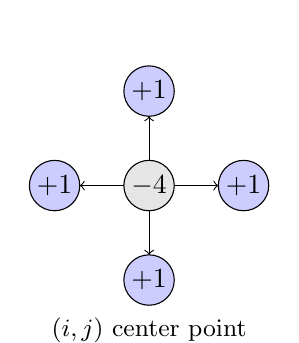
\begin{tikzpicture}[scale=0.8]
\draw[fill=gray!20] (0,0) circle (0.4) node {$-4$};
\draw[fill=blue!20] (1.5,0) circle (0.4) node {$+1$};
\draw[fill=blue!20] (-1.5,0) circle (0.4) node {$+1$};
\draw[fill=blue!20] (0,1.5) circle (0.4) node {$+1$};
\draw[fill=blue!20] (0,-1.5) circle (0.4) node {$+1$};
\draw[->] (0.4,0) -- (1.1,0);
\draw[->] (-0.4,0) -- (-1.1,0);
\draw[->] (0,0.4) -- (0,1.1);
\draw[->] (0,-0.4) -- (0,-1.1);
\node at (0,-2.3) {\small $(i,j)$ center point};
\end{tikzpicture}
\caption{The 5-point Laplacian stencil weights.}
\label{fig:stencil}
\end{figure}

The stencil computes a weighted average of the four neighbors minus four times the center value, all divided by $h^2$. This approximates how the curvature (Laplacian) at a point relates to its deviation from the average of its neighbors.


\subsubsection{Building the Linear System}

To solve the Poisson equation numerically, we must convert the stencil operations into a single large linear system $A\mathbf{z} = \mathbf{f}$. This requires mapping the 2D grid to a 1D vector and translating neighbor relationships into matrix entries.

Consider a simple $3 \times 3$ grid with 9 unknowns. Using row-major ordering, we assign linear index $k = i + j \cdot W$ where $W=3$ is the grid width:
\begin{center}
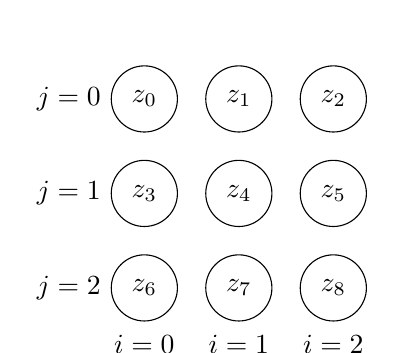
\begin{tikzpicture}[scale=1.2]
\foreach \i in {0,1,2} {
  \foreach \j in {0,1,2} {
    \pgfmathtruncatemacro{\k}{\i + \j*3}
    \draw (\i,2-\j) circle (0.35) node {$z_{\k}$};
  }
}
\node at (-0.8,2) {$j=0$};
\node at (-0.8,1) {$j=1$};
\node at (-0.8,0) {$j=2$};
\node at (0,-0.6) {$i=0$};
\node at (1,-0.6) {$i=1$};
\node at (2,-0.6) {$i=2$};
\end{tikzpicture}
\end{center}

For an interior point like $z_4$ (at position $i=1, j=1$), the 5-point stencil couples it to its four neighbors:
\begin{equation}
\frac{z_5 + z_3 + z_7 + z_1 - 4z_4}{h^2} = f_4
\end{equation}
This becomes one row of the linear system. Rearranging with unknowns on the left:
\begin{equation}
\frac{1}{h^2}z_1 + \frac{1}{h^2}z_3 - \frac{4}{h^2}z_4 + \frac{1}{h^2}z_5 + \frac{1}{h^2}z_7 = f_4
\end{equation}

Writing this for all 9 grid points simultaneously yields the matrix equation $A\mathbf{z} = \mathbf{f}$. The matrix $A$ has a characteristic block structure:
\begin{equation}
A = \frac{1}{h^2}\begin{bmatrix}
-4 & 1 & 0 & 1 & 0 & 0 & 0 & 0 & 0 \\
1 & -4 & 1 & 0 & 1 & 0 & 0 & 0 & 0 \\
0 & 1 & -4 & 0 & 0 & 1 & 0 & 0 & 0 \\
1 & 0 & 0 & -4 & 1 & 0 & 1 & 0 & 0 \\
0 & 1 & 0 & 1 & -4 & 1 & 0 & 1 & 0 \\
0 & 0 & 1 & 0 & 1 & -4 & 0 & 0 & 1 \\
0 & 0 & 0 & 1 & 0 & 0 & -4 & 1 & 0 \\
0 & 0 & 0 & 0 & 1 & 0 & 1 & -4 & 1 \\
0 & 0 & 0 & 0 & 0 & 1 & 0 & 1 & -4
\end{bmatrix}
\end{equation}

Each row corresponds to one grid point. The diagonal entry is $-4$ (center weight), entries at $\pm 1$ positions connect horizontal neighbors (same row), and entries at $\pm W$ positions connect vertical neighbors (adjacent rows). The matrix is sparse---only 5 entries per row instead of $N$---which is crucial for efficiency on large grids.

Boundary conditions modify the right-hand side $\mathbf{f}$ or the matrix structure itself. For Dirichlet conditions, known boundary values move to the right-hand side. For Neumann conditions, stencil weights at boundaries are adjusted to enforce derivative constraints. The specific modifications are detailed in the solver sections that follow.

%%%%%%%%%%%%%%%%%%%%%%%%%%%%%%%%%%%%%%%%%%%%%%%%%%%%%%
\subsection{Solver 1: FFT-Based (Spectral Method)}

The FFT-based solver exploits the fact that the Laplacian operator is diagonalized in the Fourier domain. This transforms the Poisson PDE into simple algebraic division, enabling $\mathcal{O}(N \log N)$ solution complexity. This is our fastest solver and the default choice when periodic boundary conditions are acceptable.

\subsubsection{Mathematical Approach}

The key insight is that Fourier basis functions (complex exponentials) are eigenfunctions of the Laplacian. Applying the Fourier transform to both sides of $\nabla^2 z = f$:
\begin{equation}
\mathcal{F}\{\nabla^2 z\} = \mathcal{F}\{f\}
\end{equation}
The Laplacian in the frequency domain becomes multiplication by eigenvalues. Let $\hat{Z}(\mathbf{k})$ and $\hat{F}(\mathbf{k})$ denote the Fourier transforms of $z$ and $f$ at frequency $\mathbf{k} = (k_x, k_y)$:
\begin{equation}
-|\mathbf{k}|^2 \hat{Z}(\mathbf{k}) = \hat{F}(\mathbf{k})
\end{equation}
where $|\mathbf{k}|^2 = k_x^2 + k_y^2$ is the squared frequency magnitude. Solving for the solution in frequency space:
\begin{equation}
\hat{Z}(\mathbf{k}) = \frac{\hat{F}(\mathbf{k})}{-|\mathbf{k}|^2}
\end{equation}
The solution is obtained by inverse Fourier transform:
\begin{equation}
z(x,y) = \mathcal{F}^{-1}\left\{\frac{\hat{F}(\mathbf{k})}{-|\mathbf{k}|^2}\right\}
\end{equation}
This converts the PDE (which requires solving a large linear system) into three simple operations: forward FFT, element-wise division, and inverse FFT.

\subsubsection{Boundary Condition: Periodic}

The FFT inherently assumes that the signal is periodic in all directions. This means the solver implicitly enforces:
\begin{equation}
z(0, y) = z(L_x, y), \quad z(x, 0) = z(x, L_y), \quad \text{and similarly for all derivatives}
\end{equation}
Periodic boundary conditions are rarely physical for real surfaces---few objects wrap around seamlessly at their edges. However, they work well when the object of interest is centered in the image with gradients decaying to near-zero at the boundaries.

A critical issue arises at the DC component ($\mathbf{k} = (0,0)$): the eigenvalue $|\mathbf{k}|^2 = 0$, creating a division by zero. This corresponds to the compatibility condition from Section 2.3---periodic problems determine the solution only up to an additive constant. We handle this by setting $\hat{F}[0,0] = 0$ to enforce zero-mean source (compatibility), setting the eigenvalue $\lambda[0,0] = 1$ to avoid division by zero, and the resulting $\hat{Z}[0,0] = 0$ gives a zero-mean solution.

\subsubsection{Algorithm Steps}

The complete FFT solver procedure is shown in Algorithm~\ref{alg:fft_solver}. The algorithm requires only two FFT operations (steps 2 and 6), each with $\mathcal{O}(N \log N)$ complexity, making this solver extremely fast for typical image sizes.

\begin{algorithm}[H]
\caption{FFT-Based Poisson Solver}
\label{alg:fft_solver}
\begin{algorithmic}[1]
\Require Gradient estimates $(p, q)$ from photometric stereo
\Ensure Height field $z$
\State Compute divergence: $f \gets \partial_x p + \partial_y q$
\State $\hat{F} \gets \text{FFT2D}(f)$
\State Construct eigenvalues: $\lambda_{k_x,k_y} \gets -4\pi^2(k_x^2/L_x^2 + k_y^2/L_y^2)$
\State Handle DC component: $\lambda[0,0] \gets 1$; $\hat{F}[0,0] \gets 0$
\State $\hat{Z} \gets \hat{F} / \lambda$
\State $z \gets \text{IFFT2D}(\hat{Z})$
\State $z \gets \text{Re}(z)$
\State \Return $z$
\end{algorithmic}
\end{algorithm}

%%%%%%%%%%%%%%%%%%%%%%%%%%%%%%%%%%%%%%%%%%%%%%%%%%%%%%
\newpage
\subsection{Solver 2: Finite Difference (Dirichlet Boundaries)}

The finite difference solver with Dirichlet boundary conditions constructs and solves the sparse linear system $A\mathbf{z} = \mathbf{f}$ derived in Section 3.1. Unlike the FFT approach, this method uses iterative linear algebra solvers that exploit the matrix sparsity, making it less efficient but more flexible in handling boundary conditions.

\subsubsection{Mathematical Approach}

We solve the discrete Poisson equation using the 5-point stencil developed in Section 3.1. For interior grid points, the stencil equation is:
\begin{equation}
\frac{z_{i+1,j} + z_{i-1,j} + z_{i,j+1} + z_{i,j-1} - 4z_{i,j}}{h^2} = f_{i,j}
\end{equation}
This produces a sparse $N \times N$ linear system where $N = H \cdot W$ is the total number of grid points. The matrix $A$ is symmetric negative definite, guaranteeing convergence of iterative methods.

We solve this system using the Conjugate Gradient (CG) method, an iterative algorithm that finds the solution by successively minimizing the quadratic form $\frac{1}{2}\mathbf{z}^T A \mathbf{z} - \mathbf{f}^T \mathbf{z}$. CG generates a sequence of search directions that are mutually conjugate (orthogonal with respect to $A$), ensuring that each iteration makes progress in a new direction. For symmetric positive definite systems, CG converges in at most $N$ iterations, though in practice far fewer iterations are needed when the matrix is well-conditioned.

Rather than explicitly forming the matrix $A$ (which would require storing $5N$ entries), we define a matrix-free linear operator that applies the 5-point stencil to any input vector. This reduces memory usage from $\mathcal{O}(N)$ to $\mathcal{O}(1)$ for the operator itself and enables efficient matrix-vector products.


\subsubsection{Boundary Condition: Fixed Values}

Dirichlet conditions prescribe the solution value on the boundary:
\begin{equation}
z(x,y) = g(x,y), \quad (x,y) \in \partial\Omega
\end{equation}
In the homogeneous case ($g \equiv 0$), the surface is pinned to zero height along the entire boundary. For photometric stereo, this is appropriate when the reconstructed object sits on a flat background or when the region of interest is masked to exclude edge artifacts.

Implementation is straightforward: boundary points are held fixed at the prescribed value $g$, and only interior points are solved. The stencil at interior points adjacent to boundaries incorporates the known boundary values into the right-hand side. Figure~\ref{fig:dirichlet_stencil} illustrates this for a point near the boundary.

\begin{figure}[h]
\centering
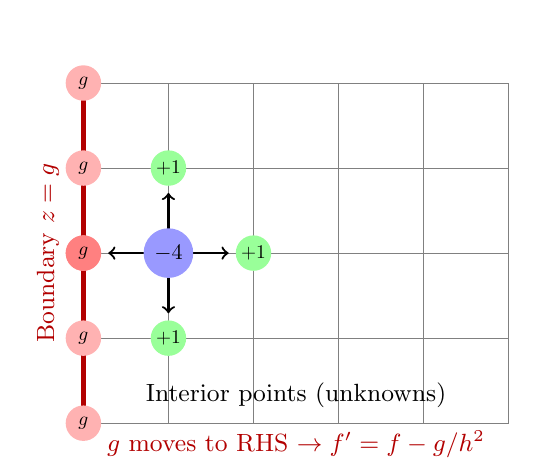
\begin{tikzpicture}[scale=0.9]
% Grid
\draw[step=1.2cm,gray,very thin] (0,0) grid (6,4.8);

% Boundary (left edge)
\draw[line width=2pt,red!70!black] (0,0) -- (0,4.8);
\node[red!70!black] at (-0.5,2.4) {\rotatebox{90}{\small Boundary $z=g$}};

% Boundary points
\foreach \j in {0,1,2,3,4} {
  \fill[red!30] (0,\j*1.2) circle (0.25);
  \node[scale=0.7] at (0,\j*1.2) {$g$};
}


% Neighbors
\fill[green!40] (2.4,2.4) circle (0.25);
\node[scale=0.7] at (2.4,2.4) {$+1$};
\fill[green!40] (1.2,3.6) circle (0.25);
\node[scale=0.7] at (1.2,3.6) {$+1$};
\fill[green!40] (1.2,1.2) circle (0.25);
\node[scale=0.7] at (1.2,1.2) {$+1$};

% Boundary neighbor (known)
\fill[red!50] (0,2.4) circle (0.25);
\node[scale=0.7] at (0,2.4) {$g$};

% Arrows
\draw[->,thick] (1.2,2.4) -- (0.35,2.4);
\draw[->,thick] (1.2,2.4) -- (2.05,2.4);
\draw[->,thick] (1.2,2.4) -- (1.2,3.25);
\draw[->,thick] (1.2,2.4) -- (1.2,1.55);

% Interior point being solved
\fill[blue!40] (1.2,2.4) circle (0.35);
\node[scale=0.8] at (1.2,2.4) {$-4$};

% Labels
\node at (3,0.4) {\small Interior points (unknowns)};
\node[red!70!black] at (3,-0.3) {\small $g$ moves to RHS $\rightarrow f' = f - g/h^2$};
\end{tikzpicture}
\caption{Dirichlet boundary conditions: The known boundary value $g$ (red) is incorporated into the right-hand side, and only interior points (blue) are solved as unknowns.}
\label{fig:dirichlet_stencil}
\end{figure}

For a point next to the left boundary ($i=1$), the stencil becomes:
\begin{equation}
\frac{z_{2,j} + g_{0,j} + z_{1,j+1} + z_{1,j-1} - 4z_{1,j}}{h^2} = f_{1,j}
\end{equation}
The known boundary value $g_{0,j}$ moves to the right-hand side: $f'_{1,j} = f_{1,j} - g_{0,j}/h^2$. This effectively reduces the system size to interior points only.

\subsubsection{Algorithm Steps}

The complete finite difference Dirichlet solver is shown in Algorithm~\ref{alg:fd_dirichlet}. The solver uses Conjugate Gradient (CG) for symmetric positive definite systems or GMRES for general sparse systems. The computational cost is $\mathcal{O}(N \cdot k)$ where $k$ is the number of CG iterations needed for convergence. Typically $k \ll N$, but the method is slower than FFT for large grids. The advantage is the ability to enforce exact boundary values.

\begin{algorithm}[H]
\caption{Finite Difference Poisson Solver (Dirichlet BC)}
\label{alg:fd_dirichlet}
\begin{algorithmic}[1]
\Require Gradient estimates $(p, q)$, boundary values $g$
\Ensure Height field $z$ with $z|_{\partial\Omega} = g$
\State Compute divergence: $f \gets \partial_x p + \partial_y q$
\State Define matrix-free operator $A: z \mapsto \nabla^2_h z$ (5-point stencil)
\State Modify RHS for boundary: $\mathbf{f}' \gets \mathbf{f} - A_{\text{boundary}} \mathbf{g}$
\State Initialize: $z_0 \gets 0$ for interior points
\State Solve: $\mathbf{z}_{\text{int}} \gets \text{CG}(A_{\text{int}}, \mathbf{f}', z_0, \text{tol})$
\State Combine: $z \gets z_{\text{int}} \cup g$
\State \Return $z$
\end{algorithmic}
\end{algorithm}

%%%%%%%%%%%%%%%%%%%%%%%%%%%%%%%%%%%%%%%%%%%%%%%%%%%%%%
\newpage
\subsection{Solver 3: Finite Difference (Neumann Boundaries)}

The Neumann solver handles problems where boundary derivatives, rather than values, are specified. This is often more physically realistic for photometric stereo, where we typically have no information about the absolute height at image boundaries---only the surface gradients.

\subsubsection{Mathematical Approach}

As with the Dirichlet solver, we discretize using the 5-point stencil and solve the resulting sparse system with Conjugate Gradient. The key difference lies in how boundary points are handled: instead of prescribing $z = g$ at boundaries, we prescribe the normal derivative $\partial z / \partial n = h$.

For homogeneous Neumann conditions ($h = 0$), the surface gradient perpendicular to the boundary is zero---the surface approaches the boundary ``flat." This is enforced by using one-sided differences at boundary points or by introducing ghost points outside the domain that mirror interior values.

A crucial distinction from the Dirichlet case is that Neumann problems with homogeneous conditions determine the solution only up to an additive constant. The compatibility condition (Section 2.3) requires:
\begin{equation}
\iint_\Omega f \, dA = 0
\end{equation}
If the source term $f$ does not integrate to zero, we subtract its mean before solving. After obtaining the solution, we typically enforce zero mean to fix the arbitrary constant.

\subsubsection{Boundary Condition: Zero Flux}

Zero-flux (homogeneous Neumann) conditions prescribe:
\begin{equation}
\frac{\partial z}{\partial n}\bigg|_{\partial\Omega} = 0
\end{equation}
This means the surface has zero slope perpendicular to the boundary. For photometric stereo, this is appropriate when we have no prior knowledge about boundary heights and want the solution to extend naturally beyond the image frame.
Using the ghost point $z_{-1,j} = z_{1,j}$ (mirroring across the boundary), the stencil at a left boundary point becomes:
\begin{equation}
\frac{z_{1,j} + z_{-1,j} + z_{0,j+1} + z_{0,j-1} - 4z_{0,j}}{h^2} = \frac{2z_{1,j} + z_{0,j+1} + z_{0,j-1} - 4z_{0,j}}{h^2} = f_{0,j}
\end{equation}
The coefficient on the interior neighbor doubles, effectively reflecting the gradient condition.

\subsubsection{Algorithm Steps}

The complete finite difference Neumann solver is shown in Algorithm~\ref{alg:fd_neumann}. The key differences from the Dirichlet solver are: (1) enforcing compatibility by subtracting the mean of $f$, (2) using the Neumann stencil at boundaries, and (3) centering the solution afterward. The computational cost remains $\mathcal{O}(N \cdot k)$.


\begin{algorithm}[H]
\caption{Finite Difference Poisson Solver (Neumann BC)}
\label{alg:fd_neumann}
\begin{algorithmic}[1]
\Require Gradient estimates $(p, q)$ from photometric stereo
\Ensure Height field $z$ with $\partial z/\partial n|_{\partial\Omega} = 0$
\State Compute divergence: $f \gets \partial_x p + \partial_y q$
\State Enforce compatibility: $f \gets f - \text{mean}(f)$
\State Define operator $A: z \mapsto \nabla^2_h z$ with Neumann stencil at boundaries
\State Initialize: $z_0 \gets 0$
\State Solve: $\mathbf{z} \gets \text{CG}(A, \mathbf{f}, z_0, \text{tol})$
\State Center solution: $z \gets z - \text{mean}(z)$
\State \Return $z$
\end{algorithmic}
\end{algorithm}

%%%%%%%%%%%%%%%%%%%%%%%%%%%%%%%%%%%%%%%%%%%%%%%%%%%%%%
\newpage
\subsection{Regularization (Noise Handling)}

Real photometric stereo data contains noise from sensor limitations, lighting imperfections, and violations of the Lambertian assumption. This noise propagates through the gradient estimation and into the Poisson problem, where it can cause severe artifacts in the reconstructed surface. Regularization techniques address this by penalizing solutions that fit noise too closely.

\subsubsection{Why Regularization is Needed}

The Poisson equation solvers developed above find the exact solution to $\nabla^2 z = f$. However, when $f$ is contaminated with noise, the ``exact'' solution faithfully reproduces that noise---often with amplification. Consider the frequency-domain solution:
\begin{equation}
\hat{Z}(\mathbf{k}) = \frac{\hat{F}(\mathbf{k})}{-|\mathbf{k}|^2}
\end{equation}
Low-frequency noise components (small $|\mathbf{k}|$) are divided by small eigenvalues, dramatically amplifying their contribution to the solution. A small amount of low-frequency noise in the gradient field can produce large-scale undulations in the reconstructed surface.

This is a manifestation of the Poisson equation's ill-conditioning for noisy data. The problem is well-posed mathematically but numerically unstable: small perturbations in $f$ cause large perturbations in $z$. Regularization stabilizes the problem by trading exact data fitting for solution smoothness.

\subsubsection{Tikhonov Derivation}

Tikhonov regularization adds a penalty term to the objective function, preferring solutions with small norm:
\begin{equation}
z_\lambda = \arg\min_z \left\{ \|\nabla^2 z - f\|^2 + \lambda \|z\|^2 \right\}
\end{equation}
The first term ensures the solution approximately satisfies the Poisson equation; the second term penalizes large height values. The parameter $\lambda > 0$ controls the trade-off: larger $\lambda$ produces smoother but less accurate solutions.

To find the minimizer, we take the first variation with respect to $z$ and set it to zero, applying the calculus of variations to the biharmonic operator that arises from composing the Laplacian with itself:
\begin{equation}
(\nabla^4 + \lambda I) z = \nabla^2 f
\end{equation}
In the frequency domain, this becomes:
\begin{equation}
\hat{Z}_\lambda(\mathbf{k}) = \frac{-|\mathbf{k}|^2 \hat{F}(\mathbf{k})}{|\mathbf{k}|^4 + \lambda}
\end{equation}

The regularization modifies the eigenvalue division: instead of dividing by $|\mathbf{k}|^2$, we effectively divide by $|\mathbf{k}|^2 + \lambda/|\mathbf{k}|^2$. This prevents blow-up at low frequencies while preserving high-frequency detail where eigenvalues are large. The regularized solution smoothly interpolates between no modification (high frequencies) and strong damping (low frequencies).

\subsubsection{Choosing the Parameter}

The regularization parameter $\lambda$ must balance bias against variance. Too small, and noise dominates; too large, and genuine surface features are smoothed away. We can quantify this trade-off by examining the regularized solution's behavior as a function of $\lambda$:
\begin{equation}
\hat{Z}_\lambda(\mathbf{k}) = \underbrace{\frac{|\mathbf{k}|^4}{|\mathbf{k}|^4 + \lambda}}_{\text{filter factor}} \cdot \hat{Z}_{\text{true}}(\mathbf{k}) + \text{noise contribution}
\end{equation}
The filter factor approaches 1 for $|\mathbf{k}|^4 \gg \lambda$ (high frequencies, no filtering) and approaches 0 for $|\mathbf{k}|^4 \ll \lambda$ (low frequencies, strong damping). Several methods exist for selecting $\lambda$.

\subsubsection{L-Curve Method}

The L-curve method provides a graphical approach to parameter selection that does not require prior knowledge of the noise level. For each candidate $\lambda$, we compute both the residual norm (how well the solution fits the data) and the solution norm (how smooth the solution is), plotting them parametrically:
\begin{equation}
\text{L-curve}: \quad \left( \log \|\nabla^2 z_\lambda - f\|, \; \log \|z_\lambda\| \right) \quad \text{for } \lambda \in [\lambda_{\min}, \lambda_{\max}]
\end{equation}

The resulting curve typically has an L-shape: for small $\lambda$ (under-regularization), the residual is small but the solution norm is large (noisy); for large $\lambda$ (over-regularization), the solution is smooth but the residual is large. The optimal $\lambda$ lies at the ``corner'' of this L-shaped curve, where the curvature:
\begin{equation}
\kappa(\lambda) = \frac{\rho'(\lambda) \eta''(\lambda) - \rho''(\lambda) \eta'(\lambda)}{(\rho'^2 + \eta'^2)^{3/2}}
\end{equation}
is maximized, where $\rho(\lambda) = \log \|\nabla^2 z_\lambda - f\|$ and $\eta(\lambda) = \log \|z_\lambda\|$. This corner represents the best trade-off between fitting the data and obtaining a smooth solution.

\subsubsection{Discrepancy Principle}

When the noise statistics are known or can be estimated, the discrepancy principle provides a principled approach to parameter selection. The key idea is that we should not fit the data more accurately than the noise allows---doing so means we are fitting noise rather than signal.

If the noise standard deviation is $\sigma$ and there are $N$ data points, the expected squared norm of the noise is $N\sigma^2$. We choose $\lambda$ such that the residual matches this expected noise level:
\begin{equation}
\|\nabla^2 z_\lambda - f\|^2 \approx N \sigma^2
\end{equation}

In practice, we solve for $\lambda$ by monotonically decreasing $\lambda$ from a large value until the residual first drops below the threshold $\tau = \sigma \sqrt{N}$. A safety factor is sometimes included:
\begin{equation}
\|\nabla^2 z_\lambda - f\| \leq \tau \cdot \delta, \quad \delta \in [1, 2]
\end{equation}
The discrepancy principle is particularly useful when the noise level can be estimated from the data itself, such as from flat regions of the image or from repeated measurements.

\subsubsection{Cross-Validation}

Cross-validation uses data splitting to estimate how well a particular $\lambda$ will generalize to unseen data. This approach is especially valuable when the noise characteristics are unknown or non-Gaussian.

Partition the data into $K$ folds (typically $K = 5$ or $K = 10$). For each fold $k$, hold out that portion of the data, fit the regularized solution $z_\lambda^{(-k)}$ using the remaining data, and compute the prediction error on the held-out set:
\begin{equation}
\text{CV}(\lambda) = \frac{1}{K} \sum_{k=1}^{K} \|z_\lambda^{(-k)} - z_{\text{test}}^{(k)}\|^2
\end{equation}
Select the regularization parameter that minimizes the cross-validation error:
\begin{equation}
\lambda^* = \arg\min_\lambda \text{CV}(\lambda)
\end{equation}

Leave-one-out cross-validation (LOOCV, $K = N$) provides an unbiased estimate but is computationally expensive. Generalized cross-validation (GCV) provides an efficient approximation for linear problems:
\begin{equation}
\text{GCV}(\lambda) = \frac{\|\nabla^2 z_\lambda - f\|^2 / N}{(1 - \text{tr}(A_\lambda)/N)^2}
\end{equation}
where $A_\lambda$ is the influence matrix mapping data to predictions.

In practice for photometric stereo, a reasonable starting point is $\lambda \approx 10^{-4}$ to $10^{-2}$, adjusted visually based on the smoothness of the reconstructed surface.


%%%%%%%%%%%%%%%%%%%%%%%%%%%%%%%%%%%%%%%%%%%%%%%%%%%%%%
% End of Chapter 3: Numerical Methods

%%%%%%%%%%%%%%%%%%%%%%%%%%%%%%%%%%%%%%%%%%%%%%%%%%%%%%
% CHAPTER 4: IMPLEMENTATION
%%%%%%%%%%%%%%%%%%%%%%%%%%%%%%%%%%%%%%%%%%%%%%%%%%%%%%

\newpage
\section{Implementation}

This chapter presents the algorithmic implementation of the photometric stereo pipeline. We focus on the computational steps required to go from raw images to a reconstructed 3D surface, emphasizing the data flow and key algorithmic decisions at each stage. The implementation integrates the mathematical foundations from Chapter 2 with the numerical solvers from Chapter 3.

\subsection{Photometric Stereo Pipeline}

The complete pipeline consists of four stages: image acquisition and preprocessing, light matrix construction, per-pixel normal estimation, and gradient field computation. Algorithm~\ref{alg:pipeline} provides an overview.

\begin{algorithm}[H]
\caption{Photometric Stereo Pipeline}
\label{alg:pipeline}
\begin{algorithmic}[1]
\Require Images $\{I_1, \ldots, I_K\}$ under known lighting $\{\mathbf{l}_1, \ldots, \mathbf{l}_K\}$
\Ensure Reconstructed height field $z(x,y)$
\State Preprocess images: normalization, background subtraction
\State Construct light matrix $L \in \mathbb{R}^{K \times 3}$
\State \textbf{for} each pixel $(x,y)$ \textbf{do}
\State \quad Solve $L \mathbf{n} = \mathbf{i}$ for surface normal $\mathbf{n}(x,y)$
\State \textbf{end for}
\State Compute gradients: $p = -n_x/n_z$, $q = -n_y/n_z$
\State Compute divergence: $f = \partial_x p + \partial_y q$
\State Solve Poisson equation: $\nabla^2 z = f$
\State \Return $z$
\end{algorithmic}
\end{algorithm}

\subsubsection{Image Acquisition and Preprocessing}

The input consists of $K$ grayscale images of a static scene, each captured under a different known lighting direction. For reliable normal estimation, we require $K \geq 3$ non-coplanar light sources, though $K = 4$ to $8$ provides better noise robustness.

Several preprocessing steps are essential for high-quality reconstruction. First, intensity normalization converts raw pixel values to the range $[0, 1]$ and applies gamma correction if the camera response is nonlinear. Second, background subtraction removes ambient illumination by subtracting an image captured with all lights off, or by estimating a low-frequency background model. Third, shadow detection identifies pixels where the surface is in shadow (intensity below a threshold); these measurements violate the Lambertian model and should be excluded from the least-squares fit. Finally, saturation handling excludes pixels at maximum intensity, as they provide no gradient information.

For each pixel location $(x,y)$, we collect the intensity vector:
\begin{equation}
\mathbf{i}(x,y) = [I_1(x,y), I_2(x,y), \ldots, I_K(x,y)]^T
\end{equation}


\subsubsection{Light Matrix Construction}

The lighting directions must be known or calibrated. Each light direction $\mathbf{l}_k = (\ell_{k,x}, \ell_{k,y}, \ell_{k,z})^T$ is a unit vector pointing from the surface toward the light source. These are assembled into the light matrix:
\begin{equation}
L = \begin{bmatrix}
\ell_{1,x} & \ell_{1,y} & \ell_{1,z} \\
\ell_{2,x} & \ell_{2,y} & \ell_{2,z} \\
\vdots & \vdots & \vdots \\
\ell_{K,x} & \ell_{K,y} & \ell_{K,z}
\end{bmatrix} \in \mathbb{R}^{K \times 3}
\end{equation}

For well-conditioned normal estimation, the light directions should span 3D space. The condition number $\kappa(L^T L)$ indicates sensitivity to noise---lower is better. Optimal configurations distribute lights uniformly over the hemisphere, avoiding coplanar arrangements.

Common calibration methods include using a reference sphere with known geometry (the ``chrome ball'' technique) or directly measuring light positions with a goniometer.

\subsubsection{Per-Pixel Normal Estimation}

At each pixel, we solve the overdetermined system $L \mathbf{n} = \mathbf{i}$ for the surface normal $\mathbf{n}$. The Lambertian model gives:
\begin{equation}
I_k(x,y) = \rho(x,y) \cdot \mathbf{l}_k \cdot \mathbf{n}(x,y)
\end{equation}
where $\rho$ is the albedo (reflectivity) at that pixel. We solve for the product $\mathbf{m} = \rho \mathbf{n}$ using least squares:
\begin{equation}
\mathbf{m}^* = (L^T L)^{-1} L^T \mathbf{i} = L^\dagger \mathbf{i}
\end{equation}
where $L^\dagger$ is the Moore-Penrose pseudoinverse. The albedo and normal are then separated:
\begin{equation}
\rho = \|\mathbf{m}^*\|, \quad \mathbf{n} = \frac{\mathbf{m}^*}{\|\mathbf{m}^*\|}
\end{equation}

For pixels with shadows or specular highlights, robust estimation methods (e.g., RANSAC or iteratively reweighted least squares) can improve results by down-weighting outlier measurements.

\subsubsection{Gradient Field Computation}

Given the surface normal $\mathbf{n} = (n_x, n_y, n_z)^T$ at each pixel, we extract the surface gradients. Under the assumption that $z = z(x,y)$ is a height field, the normal vector is:
\begin{equation}
\mathbf{n} = \frac{1}{\sqrt{1 + p^2 + q^2}} \begin{pmatrix} -p \\ -q \\ 1 \end{pmatrix}
\end{equation}
where $p = \partial z / \partial x$ and $q = \partial z / \partial y$. Rearranging:
\begin{equation}
p = -\frac{n_x}{n_z}, \quad q = -\frac{n_y}{n_z}
\end{equation}

This conversion requires $n_z > 0$ (surface visible from above). Pixels where $n_z \leq 0$ correspond to overhanging surfaces or self-occlusion and cannot be reconstructed as a height field.

The gradient fields $(p, q)$ are then passed to the Poisson solvers from Chapter 3. The divergence is computed using central differences:
\begin{equation}
f_{i,j} = \frac{p_{i+1,j} - p_{i-1,j}}{2h} + \frac{q_{i,j+1} - q_{i,j-1}}{2h}
\end{equation}

%%%%%%%%%%%%%%%%%%%%%%%%%%%%%%%%%%%%%%%%%%%%%%%%%%%%%%
\subsection{Poisson Solver Integration}

Once the gradient fields $(p, q)$ are computed from the surface normals, the next stage integrates these gradients to recover the height field $z(x,y)$. This involves constructing the divergence field, selecting an appropriate Poisson solver based on boundary conditions, and post-processing the result.

\subsubsection{Divergence Field Construction}

The Poisson equation $\nabla^2 z = f$ requires the right-hand side $f$ to be the divergence of the gradient field. Using central differences on a grid with spacing $h$:
\begin{equation}
f_{i,j} = \frac{\partial p}{\partial x}\bigg|_{i,j} + \frac{\partial q}{\partial y}\bigg|_{i,j} \approx \frac{p_{i+1,j} - p_{i-1,j}}{2h} + \frac{q_{i,j+1} - q_{i,j-1}}{2h}
\end{equation}

At boundary pixels, one-sided differences are used. For the left boundary ($i = 0$):
\begin{equation}
\frac{\partial p}{\partial x}\bigg|_{0,j} \approx \frac{p_{1,j} - p_{0,j}}{h}
\end{equation}
and similarly for other edges and corners. The divergence computation can be implemented efficiently using convolution with appropriate finite difference kernels.

Missing or invalid pixels (shadows, specular highlights, or regions where $n_z \leq 0$) are marked in a validity mask. The Poisson solver can either interpolate over these regions or treat them as internal Dirichlet constraints.

\subsubsection{Solver Selection Logic}

The choice of Poisson solver depends on the desired boundary conditions and computational constraints. Algorithm~\ref{alg:solver_select} summarizes the selection logic.

\begin{algorithm}[H]
\caption{Poisson Solver Selection}
\label{alg:solver_select}
\begin{algorithmic}[1]
\Require Divergence field $f$, boundary condition type, regularization parameter $\lambda$
\Ensure Height field $z$
\If{boundary\_type = PERIODIC}
    \State $z \gets \text{FFT\_Solver}(f)$ \Comment{$\mathcal{O}(N \log N)$}
\ElsIf{boundary\_type = DIRICHLET}
    \State $z \gets \text{FD\_Dirichlet\_Solver}(f, g)$ \Comment{CG on interior}
\ElsIf{boundary\_type = NEUMANN}
    \State $f \gets f - \text{mean}(f)$ \Comment{Enforce compatibility}
    \State $z \gets \text{FD\_Neumann\_Solver}(f)$ \Comment{CG with modified stencil}
\EndIf
\If{$\lambda > 0$}
    \State Apply Tikhonov regularization during solve
\EndIf
\State \Return $z$
\end{algorithmic}
\end{algorithm}

For most photometric stereo applications, the FFT solver provides the best balance of speed and accuracy when the object is centered in the image with gradients decaying near the boundaries. When exact boundary control is needed (e.g., object on a known flat plane), the Dirichlet solver is preferred. The Neumann solver is appropriate when boundary heights are unknown but should vary smoothly.

\subsubsection{Post-Processing (Mean Centering)}

The recovered height field $z$ is determined only up to an additive constant for both periodic and Neumann boundary conditions. We fix this ambiguity by enforcing zero mean:
\begin{equation}
z_{\text{centered}} = z - \frac{1}{N} \sum_{i,j} z_{i,j}
\end{equation}
where $N$ is the total number of valid pixels. This centers the surface around the $z = 0$ plane.

Additional post-processing steps may include median filtering to remove isolated spike artifacts, clipping extreme values that arise from noisy gradient estimates, or applying a low-pass filter to smooth high-frequency reconstruction noise. For visualization, the height field is typically scaled to a convenient range and rendered as a 3D mesh or depth map.

%%%%%%%%%%%%%%%%%%%%%%%%%%%%%%%%%%%%%%%%%%%%%%%%%%%%%%
\newpage
\subsection{Software Architecture Overview}

\textbf{[STUB SECTION --- TO BE REWRITTEN]}

This section provides an overview of the software architecture for both Python and MATLAB implementations. The modular design separates concerns into distinct components for image processing, normal estimation, and surface reconstruction.

\subsubsection{Python Implementation Structure}

\textbf{[PLACEHOLDER --- CONTENT TO BE REPLACED]}

The Python implementation follows a modular architecture organized into the following components. Figure~\ref{fig:python_arch_stub} shows a placeholder diagram.

\begin{figure}[H]
\centering
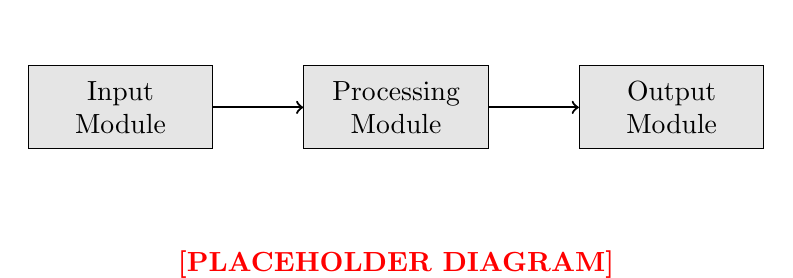
\begin{tikzpicture}[node distance=1.5cm, auto,
    block/.style={rectangle, draw, fill=gray!20, text width=6em, text centered, minimum height=3em},
    arrow/.style={->, thick}]
    
    \node[block] (input) {Input Module};
    \node[block, right of=input, xshift=2cm] (process) {Processing Module};
    \node[block, right of=process, xshift=2cm] (output) {Output Module};
    
    \draw[arrow] (input) -- (process);
    \draw[arrow] (process) -- (output);
    
    \node[below of=process, yshift=-0.5cm, text=red] {\textbf{[PLACEHOLDER DIAGRAM]}};
\end{tikzpicture}
\caption{Python module architecture (STUB --- to be replaced with actual implementation details).}
\label{fig:python_arch_stub}
\end{figure}

Lorem ipsum dolor sit amet, consectetur adipiscing elit. Sed do eiusmod tempor incididunt ut labore et dolore magna aliqua. Ut enim ad minim veniam, quis nostrud exercitation ullamco laboris.

\subsubsection{MATLAB Implementation Structure}

\textbf{[PLACEHOLDER --- CONTENT TO BE REPLACED]}

The MATLAB implementation provides a reference implementation with similar functionality. Figure~\ref{fig:matlab_arch_stub} shows the placeholder architecture.

\begin{figure}[H]
\centering
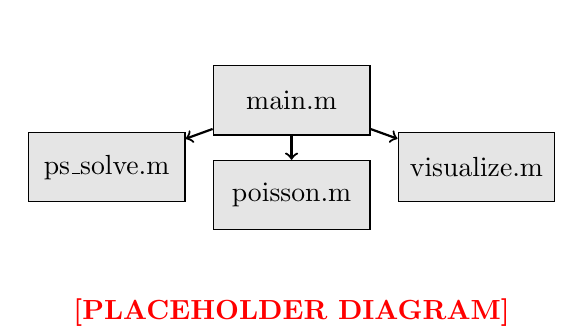
\begin{tikzpicture}[node distance=1.2cm, auto,
    block/.style={rectangle, draw, fill=gray!20, text width=5em, text centered, minimum height=2.5em},
    arrow/.style={->, thick}]
    
    \node[block] (main) {main.m};
    \node[block, below left of=main, xshift=-1.5cm] (ps) {ps\_solve.m};
    \node[block, below of=main] (poisson) {poisson.m};
    \node[block, below right of=main, xshift=1.5cm] (viz) {visualize.m};
    
    \draw[arrow] (main) -- (ps);
    \draw[arrow] (main) -- (poisson);
    \draw[arrow] (main) -- (viz);
    
    \node[below of=poisson, yshift=-0.3cm, text=red] {\textbf{[PLACEHOLDER DIAGRAM]}};
\end{tikzpicture}
\caption{MATLAB function hierarchy (STUB --- to be replaced with actual code structure).}
\label{fig:matlab_arch_stub}
\end{figure}

Duis aute irure dolor in reprehenderit in voluptate velit esse cillum dolore eu fugiat nulla pariatur. Excepteur sint occaecat cupidatat non proident.

\subsubsection{Code Validation Strategy}

\textbf{[PLACEHOLDER --- CONTENT TO BE REPLACED]}

Validation of the implementation involves several strategies shown in Figure~\ref{fig:validation_stub}.

\begin{figure}[H]
\centering
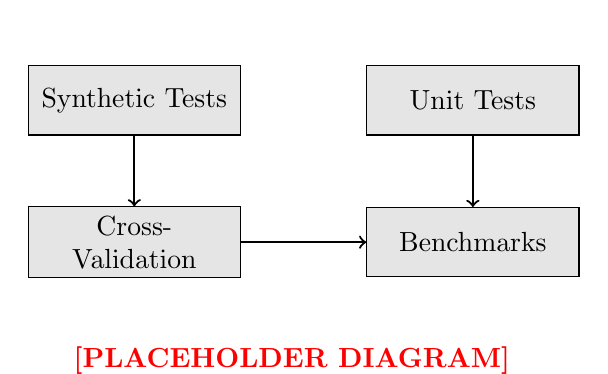
\begin{tikzpicture}[node distance=1.8cm, auto,
    block/.style={rectangle, draw, fill=gray!20, text width=7em, text centered, minimum height=2.5em},
    arrow/.style={->, thick}]
    
    \node[block] (synth) {Synthetic Tests};
    \node[block, right of=synth, xshift=2.5cm] (unit) {Unit Tests};
    \node[block, below of=synth] (compare) {Cross-Validation};
    \node[block, below of=unit] (bench) {Benchmarks};
    
    \draw[arrow] (synth) -- (compare);
    \draw[arrow] (unit) -- (bench);
    \draw[arrow] (compare) -- (bench);
    
    \node[below of=compare, xshift=2cm, yshift=0.3cm, text=red] {\textbf{[PLACEHOLDER DIAGRAM]}};
\end{tikzpicture}
\caption{Validation workflow (STUB --- to be replaced with actual testing methodology).}
\label{fig:validation_stub}
\end{figure}

Sed ut perspiciatis unde omnis iste natus error sit voluptatem accusantium doloremque laudantium, totam rem aperiam, eaque ipsa quae ab illo inventore veritatis.

%%%%%%%%%%%%%%%%%%%%%%%%%%%%%%%%%%%%%%%%%%%%%%%%%%%%%%
% End of Chapter 4: Implementation

%%%%%%%%%%%%%%%%%%%%%%%%%%%%%%%%%%%%%%%%%%%%%%%%%%%%%%
% CHAPTER 5: EXPERIMENTAL VALIDATION
%%%%%%%%%%%%%%%%%%%%%%%%%%%%%%%%%%%%%%%%%%%%%%%%%%%%%%

\newpage
\section{Experimental Validation}

This chapter presents experimental results validating the photometric stereo pipeline and Poisson solvers. We use synthetic test surfaces with known ground truth to evaluate reconstruction accuracy, enabling quantitative error analysis. The experiments compare solver performance across different boundary conditions, noise levels, and surface geometries.

\subsection{Test Surfaces}

Validation requires surfaces with analytically known height fields $z(x,y)$ so reconstruction errors can be measured precisely. We define a suite of test surfaces that span different geometric characteristics---smooth and peaked, convex and saddle-shaped, single-scale and multi-frequency.

\subsubsection{Surface Selection Rationale}

We selected eight synthetic surfaces that stress different aspects of the pipeline: smooth, radially symmetric shapes (Gaussian bump, hemisphere, ellipsoid, soft cone) reveal how well integration preserves curvature and absolute depth; piecewise-linear or sign-changing geometries (softened cube, saddle) probe sensitivity to sharp edges and mixed second derivatives; periodic or multi-modal landscapes (sinusoidal, MATLAB Peaks) stress global consistency.

Figure~\ref{fig:test_surfaces} provides a visualization of these geometries, and Table~\ref{tab:test_surface_formulas} gives their analytical definitions.

\begin{figure}[H]
\centering
\includegraphics[width=0.95\textwidth]{surfaces}
\caption{Eight synthetic surfaces used: (a) Gaussian bump, (b) hemisphere, (c) softened cube, (d) ellipsoid, (e) sinusoidal, (f) soft cone, (g) saddle, and (h) MATLAB Peaks.}
\label{fig:test_surfaces}
\end{figure}

\begin{table}[H]
\centering
\caption{Analytical definitions of the benchmark surfaces.}
\label{tab:test_surface_formulas}
\renewcommand{\arraystretch}{1.5}
\begin{tabularx}{\textwidth}{lX}
\hline\hline
\textbf{Surface} & \textbf{Height function $z(x,y)$} \\
\hline
Gaussian bump & $\exp\!\left(-\dfrac{x^2+y^2}{2\sigma^2}\right)$, $\sigma = 0.4$ \\
Hemisphere & $\sqrt{R^2 - (x^2 + y^2)}$ for $x^2 + y^2 \le R^2$, $R = 0.9$ \\
Softened cube & $0.6\,\text{clip}\!\left(1 - \dfrac{\max(|x|,|y|) - 0.45}{0.1},\,0,\,1\right)$ \\
Ellipsoid & $c\sqrt{1 - (x/a)^2 - (y/b)^2}$, $a = 0.8$, $b = 0.6$, $c = 0.5$ \\
Sinusoidal & $A \sin(\pi x)\sin(\pi y)$, $A = 0.3$ \\
Soft cone & $h \max\!\left(0, 1 - \dfrac{\sqrt{x^2 + y^2}}{R}\right)$, $h = 0.8$, $R = 0.9$ \\
Saddle & $\alpha x y$, $\alpha = 0.3$ \\
MATLAB Peaks & $3(1-x)^2 e^{-x^2-(y+1)^2} - 10\!\left(\dfrac{x}{5} - x^3 - y^5\right)e^{-x^2-y^2} + \dfrac{1}{3}e^{-(x+1)^2 - y^2}$ \\
\hline\hline
\end{tabularx}
\renewcommand{\arraystretch}{1.0}
\end{table}

Together, these surfaces provide comprehensive coverage of the geometric scenarios encountered in real photometric stereo applications.


%%%%%%%%%%%%%%%%%%%%%%%%%%%%%%%%%%%%%%%%%%%%%%%%%%%%%%
\subsection{Experimental Protocol}

To rigorously evaluate the pipeline, we follow a standardized testing protocol across all surfaces. This ensures that performance differences can be attributed to surface geometry or solver choice rather than varying implementation details.


\subsubsection{Common Setup Parameters}

Unless otherwise specified, all experiments use the default parameters listed in Table~\ref{tab:setup_params}. This standardization allows for direct comparison across different experiments.

\begin{table}[H]
\centering
\caption{Default experimental parameters used across all test surfaces.}
\label{tab:setup_params}
\renewcommand{\arraystretch}{1.3}
\begin{tabularx}{\textwidth}{lX}
\hline\hline
\textbf{Parameter} & \textbf{Configuration Details} \\
\hline
\textbf{Grid Resolution} & $128 \times 128$ pixel grid covering the domain $(x,y) \in [-1, 1] \times [-1, 1]$. This resolution captures sufficient surface detail while maintaining tractable computation times. \\
\textbf{Lighting} & A ``ring + zenith'' configuration with $K=5$ lights: four at $45^\circ$ elevation ($90^\circ$ azimuth spacing) and one overhead zenith light given by $\mathbf{l} = (0,0,1)^T$. \\
\textbf{Reflectance} & Perfect Lambertian reflectance with uniform unit albedo ($\rho = 1.0$) and no specular highlights or cast shadows in the baseline simulations. \\
\textbf{Noise Model} & Baseline tests use ideal noise-free images. Robustness tests inject additive zero-mean Gaussian noise $\mathcal{N}(0, \sigma^2)$ to normalized pixel intensities. \\
\hline\hline
\end{tabularx}
\renewcommand{\arraystretch}{1.0}
\end{table}


\subsubsection{Evaluation Metrics}

We quantify reconstruction quality using two primary metrics: one for surface orientation and one for surface depth. It is important to present them in this order, as normal estimation errors are the causal precursor to depth reconstruction errors.

\paragraph{Mean Angular Error (MAE).}
This metric evaluates how well the surface normals are recovered, which is the direct output of the photometric stereo step. For each pixel, the angular error $\theta$ is the angle between the true normal $\mathbf{n}_{\text{gt}}$ and estimated normal $\mathbf{n}_{\text{rec}}$:
\begin{equation}
\theta(x,y) = \arccos\left( \text{clip}(\mathbf{n}_{\text{gt}} \cdot \mathbf{n}_{\text{rec}}, -1, 1) \right)
\end{equation}
We report the mean angular error over the domain in degrees:
\begin{equation}
\text{MAE} = \frac{1}{N} \sum_{(x,y) \in \Omega} \theta(x,y) \, \frac{180}{\pi}
\end{equation}
Low MAE implies accurate local slope estimation. However, even small angular biases can accumulate during integration, leading to significant low-frequency depth distortions.

\paragraph{Depth Error (RMSE).}
The Root Mean Square Error (RMSE) measures the global accuracy of the integrated surface. Since Poisson integration yields height up to an additive constant, we align the reconstruction $z_{\text{rec}}$ with the ground truth $z_{\text{gt}}$ by subtracting their means:
\begin{equation}
z'_{\text{rec}} = z_{\text{rec}} - \bar{z}_{\text{rec}}, \quad z'_{\text{gt}} = z_{\text{gt}} - \bar{z}_{\text{gt}}
\end{equation}
RMSE is then computed over all valid pixels $N$:
\begin{equation}
\text{RMSE} = \sqrt{\frac{1}{N} \sum_{(x,y) \in \Omega} (z'_{\text{rec}}(x,y) - z'_{\text{gt}}(x,y))^2}
\end{equation}
This metric captures the cumulative effect of angular errors. High RMSE alongside low MAE typically indicates a systematic bias in the normal field (e.g., ``slanting'' the entire surface) that integration amplifies over the domain.


%%%%%%%%%%%%%%%%%%%%%%%%%%%%%%%%%%%%%%%%%%%%%%%%%%%%%%
\subsection{Core Validation}\label{sec:core_validation}

This section validates the two primary software components: the Poisson solver itself (using exact gradients) and the complete photometric stereo pipeline (using rendered images).

\subsubsection{Validation 1: Poisson Solver Validation (Gradient $\rightarrow$ Height)}

We first isolate the integration step by bypassing the normal estimation entirely. Using the analytic Gaussian surface, we compute exact gradients $(p,q)$ analytically, differentiate them to form the divergence field $f$, and pass this directly to the FFT solver. This establishes the numerical floor of the method, separating integration error from photometric noise.

\begin{center}
\resizebox{0.9\linewidth}{!}{%
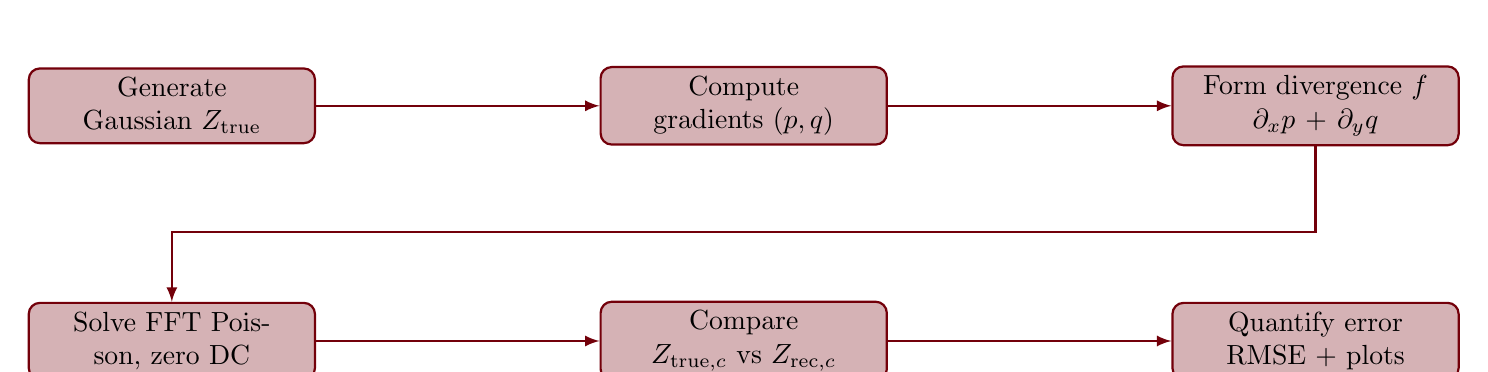
\begin{tikzpicture}[>=latex,
                    every node/.style={draw=USCGarnet, rounded corners, align=center,
                                       text width=3.4cm, fill=USCGarnet!30},
                    every path/.style={draw=USCGarnet, thick}]
\node (surf) {Generate \\Gaussian $Z_{\text{true}}$};
\node[right=3.6cm of surf] (grad) {Compute \\gradients $(p,q)$ };
\node[right=3.6cm of grad] (div) {Form divergence $f$\\ $\partial_x p + \partial_y q$};
\node[below=2.0cm of surf] (solve) {Solve FFT Poisson, zero DC};
\node[right=3.6cm of solve] (cmp) {Compare\\ $Z_{\text{true},c}$ vs $Z_{\text{rec},c}$};
\node[right=3.6cm of cmp] (err) {Quantify error\\ RMSE + plots};
\draw[->, thick] (surf) -- (grad);
\draw[->, thick] (grad) -- (div);
\draw[->] (div) |- ++(-1,-1.6) -| (solve);
\draw[->, thick] (solve) -- (cmp);
\draw[->, thick] (cmp) -- (err);
\end{tikzpicture}%
}
\end{center}

Figure~\ref{fig:exp1_layout} confirms that the solver is functioning correctly. The reconstructed surface is visually indistinguishable from the ground truth, and the error histogram is tightly concentrated around zero. The small residual errors (RMSE $\approx 2.2 \times 10^{-2}$) arise primarily from the periodic boundary assumption of the FFT solver applied to a non-periodic Gaussian patch, which creates a slight ``wrapping'' artifact at the edges.

\begin{figure}[H]
\centering
\begin{subfigure}[b]{0.23\textwidth}
\includegraphics[width=\linewidth]{exp1_3d_true.png}
\caption{True 3D}
\end{subfigure}
\begin{subfigure}[b]{0.23\textwidth}
\includegraphics[width=\linewidth]{exp1_3d_rec.png}
\caption{Reconstruction}
\end{subfigure}
\begin{subfigure}[b]{0.23\textwidth}
\includegraphics[width=\linewidth]{exp1_Z_true.png}
\caption{Ground-truth depth}
\end{subfigure}
\begin{subfigure}[b]{0.23\textwidth}
\includegraphics[width=\linewidth]{exp1_Z_rec.png}
\caption{Recovered depth}
\end{subfigure}

\bigskip
\begin{subfigure}[b]{0.23\textwidth}
\includegraphics[width=\linewidth]{exp1_error.png}
\caption{Depth error}
\end{subfigure}
\begin{subfigure}[b]{0.23\textwidth}
\includegraphics[width=\linewidth]{exp1_profile.png}
\caption{Center-line profile}
\end{subfigure}
\begin{subfigure}[b]{0.23\textwidth}
\includegraphics[width=\linewidth]{exp1_hist.png}
\caption{Error histogram}
\end{subfigure}
\caption{Validation 1 Results. Exact Gaussian gradients drive the FFT solver, yielding extremely low error and verifying the integrator implementation.}
\label{fig:exp1_layout}
\end{figure}

\subsubsection{Validation 2: Full PS Pipeline (Image $\rightarrow$ Height)}

Next, we validate the full pipeline. We render five Lambertian images of the Gaussian surface (one zenith, four oblique) and use photometric stereo to estimate the normals before integration. This introduces realistic errors associated with the least-squares normal fit.

\begin{center}
\resizebox{0.9\linewidth}{!}{%
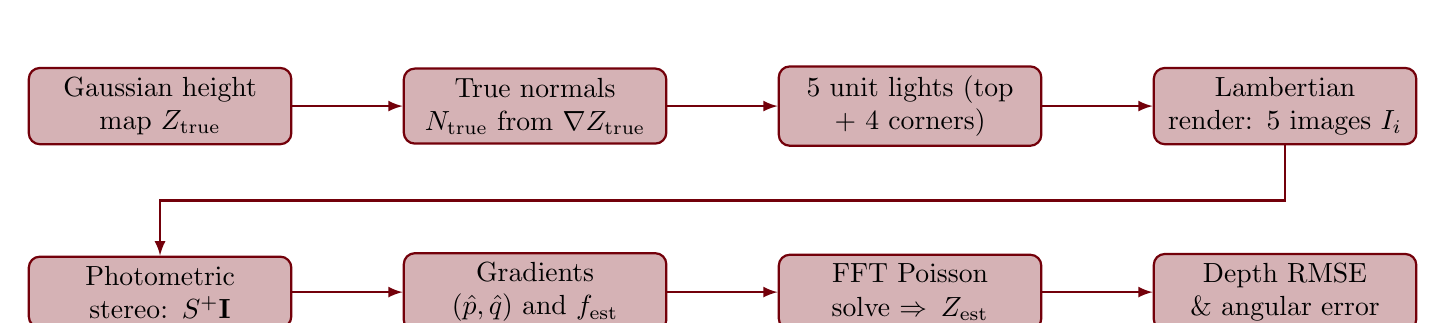
\begin{tikzpicture}[node distance=1.4cm,>=latex,
                    every node/.style={draw=USCGarnet, rounded corners, align=center,
                                       text width=3.1cm, fill=USCGarnet!30},
                    every path/.style={draw=USCGarnet, thick}]
\node (surf) {Gaussian height map $Z_{\text{true}}$};
\node[right=of surf] (normals) {True normals $N_{\text{true}}$ from $\nabla Z_{\text{true}}$};
\node[right=of normals] (lights) {5 unit lights (top + 4 corners)};
\node[right=of lights] (render) {Lambertian render: 5 images $I_i$};
\node[below=of surf] (ps) {Photometric stereo: $S^+\mathbf{I}$};
\node[right=of ps] (grads) {Gradients $(\hat{p},\hat{q})$ and $f_{\text{est}}$};
\node[right=of grads] (poisson) {FFT Poisson solve $\Rightarrow Z_{\text{est}}$};
\node[right=of poisson] (metrics) {Depth RMSE \& angular error};
\draw[->] (surf) -- (normals);
\draw[->] (normals) -- (lights);
\draw[->] (lights) -- (render);
\draw[->] (render) |- ++(-1,-1.2) -| (ps);
\draw[->] (ps) -- (grads);
\draw[->] (grads) -- (poisson);
\draw[->] (poisson) -- (metrics);
\end{tikzpicture}
}%
\end{center}

Figure~\ref{fig:exp2_layout} shows the results. The normal estimation is highly accurate in the center where all five lights illuminate the surface. Near the boundaries, grazing angles lead to slightly higher angular errors. However, the integrated surface remains robust, with an RMSE ($2.26 \times 10^{-2}$) only marginally higher than the solver-only baseline. This confirms that the least-squares normal estimation is working correctly and passing high-quality gradients to the integrator.

\begin{figure}[H]
\centering
\begin{subfigure}[b]{0.23\textwidth}
\includegraphics[width=\linewidth]{exp2_3d_true.png}
\caption{True 3D}
\end{subfigure}
\begin{subfigure}[b]{0.23\textwidth}
\includegraphics[width=\linewidth]{exp2_3d_est.png}
\caption{Reconstruction}
\end{subfigure}
\begin{subfigure}[b]{0.23\textwidth}
\includegraphics[width=\linewidth]{exp2_Z_est.png}
\caption{Recovered depth}
\end{subfigure}
\begin{subfigure}[b]{0.23\textwidth}
\includegraphics[width=\linewidth]{exp2_error.png}
\caption{Depth error}
\end{subfigure}

\bigskip
\begin{subfigure}[b]{0.23\textwidth}
\includegraphics[width=\linewidth]{exp2_normals_gt.png}
\caption{Normals (GT)}
\end{subfigure}
\begin{subfigure}[b]{0.23\textwidth}
\includegraphics[width=\linewidth]{exp2_normals_est.png}
\caption{Normals (est.)}
\end{subfigure}
\begin{subfigure}[b]{0.23\textwidth}
\includegraphics[width=\linewidth]{exp2_profile.png}
\caption{Center-line profile}
\end{subfigure}
\begin{subfigure}[b]{0.23\textwidth}
\includegraphics[width=\linewidth]{exp2_hist.png}
\caption{Depth error hist.}
\end{subfigure}
\caption{Validation 2 Results. The full pipeline achieves RMSE $=2.26\times10^{-2}$. Angular errors are suppressed across most of the dome, verifying the complete photometric stereo workflow.}
\label{fig:exp2_layout}
\end{figure}

%%%%%%%%%%%%%%%%%%%%%%%%%%%%%%%%%%%%%%%%%%%%%%%%%%%%%%
% PLACEHOLDER: Section 5.4 - Smooth Curved Surface Experiments

\end{document}